\documentclass[a4paper]{book}
\usepackage{makeidx}
\usepackage{natbib}
\usepackage{graphicx}
\usepackage{multicol}
\usepackage{float}
\usepackage{listings}
\usepackage{color}
\usepackage{ifthen}
\usepackage[table]{xcolor}
\usepackage{textcomp}
\usepackage{alltt}
\usepackage{ifpdf}
\ifpdf
\usepackage[pdftex,
            pagebackref=true,
            colorlinks=true,
            linkcolor=blue,
            unicode
           ]{hyperref}
\else
\usepackage[ps2pdf,
            pagebackref=true,
            colorlinks=true,
            linkcolor=blue,
            unicode
           ]{hyperref}
\usepackage{pspicture}
\fi
\usepackage[utf8]{inputenc}
\usepackage{mathptmx}
\usepackage[scaled=.90]{helvet}
\usepackage{courier}
\usepackage{sectsty}
\usepackage[titles]{tocloft}
\usepackage{doxygen}
\lstset{language=C++,inputencoding=utf8,basicstyle=\footnotesize,breaklines=true,breakatwhitespace=true,tabsize=8,numbers=left }
\makeindex
\setcounter{tocdepth}{3}
\renewcommand{\footrulewidth}{0.4pt}
\renewcommand{\familydefault}{\sfdefault}
\hfuzz=15pt
\setlength{\emergencystretch}{15pt}
\hbadness=750
\tolerance=750
\begin{document}
\hypersetup{pageanchor=false,citecolor=blue}
\begin{titlepage}
\vspace*{7cm}
\begin{center}
{\Large \-My \-Project }\\
\vspace*{1cm}
{\large \-Generated by Doxygen 1.7.6.1}\\
\vspace*{0.5cm}
{\small Tue Apr 21 2015 10:04:16}\\
\end{center}
\end{titlepage}
\clearemptydoublepage
\pagenumbering{roman}
\tableofcontents
\clearemptydoublepage
\pagenumbering{arabic}
\hypersetup{pageanchor=true,citecolor=blue}
\chapter{\-Main \-Page}
\label{index}\hypertarget{index}{}

{\bfseries \-C\-I\-T\-I\-U\-S\-\_\-\-Control\-\_\-\-Communication} 

-\/-\/$>$ 
\chapter{\-Class \-Index}
\section{\-Class \-Hierarchy}
\-This inheritance list is sorted roughly, but not completely, alphabetically\-:\begin{DoxyCompactList}
\item \contentsline{section}{\-Thread}{\pageref{class_thread}}{}
\begin{DoxyCompactList}
\item \contentsline{section}{\-C\-A\-N\-Communication}{\pageref{class_c_a_n_communication}}{}
\item \contentsline{section}{\-Conduccion\-Thread}{\pageref{class_conduccion_thread}}{}
\end{DoxyCompactList}
\item \contentsline{section}{\-Thread\-Exception}{\pageref{class_thread_exception}}{}
\item \contentsline{section}{\-Timer}{\pageref{class_timer}}{}
\end{DoxyCompactList}

\chapter{\-Class \-Index}
\section{\-Class \-List}
\-Here are the classes, structs, unions and interfaces with brief descriptions\-:\begin{DoxyCompactList}
\item\contentsline{section}{\hyperlink{struct_frame_driving}{\-Frame\-Driving} }{\pageref{struct_frame_driving}}{}
\item\contentsline{section}{\hyperlink{class_jaus_handler}{\-Jaus\-Handler} }{\pageref{class_jaus_handler}}{}
\item\contentsline{section}{\hyperlink{class_ros_node___communications}{\-Ros\-Node\-\_\-\-Communications} \\*\-Clase que implementa el nodo de \-Comunicaciones }{\pageref{class_ros_node___communications}}{}
\item\contentsline{section}{\hyperlink{class_translator_r_o_s_j_a_u_s}{\-Translator\-R\-O\-S\-J\-A\-U\-S} }{\pageref{class_translator_r_o_s_j_a_u_s}}{}
\end{DoxyCompactList}

\chapter{\-File \-Index}
\section{\-File \-List}
\-Here is a list of all documented files with brief descriptions\-:\begin{DoxyCompactList}
\item\contentsline{section}{include/\-Modulo\-\_\-\-Conduccion/\hyperlink{_c_a_n_communication_8hpp}{\-C\-A\-N\-Communication.\-hpp} \\*\-Declara el tipo de la clase \char`\"{}\-C\-A\-N\-Communication\char`\"{} }{\pageref{_c_a_n_communication_8hpp}}{}
\item\contentsline{section}{include/\-Modulo\-\_\-\-Conduccion/{\bfseries conduccion.\-h} }{\pageref{conduccion_8h}}{}
\item\contentsline{section}{include/\-Modulo\-\_\-\-Conduccion/\hyperlink{_conduccion_thread_8hpp}{\-Conduccion\-Thread.\-hpp} \\*\-Declara el tipo de la clase \char`\"{}\-Conduccion\-Thread\char`\"{} }{\pageref{_conduccion_thread_8hpp}}{}
\item\contentsline{section}{include/\-Modulo\-\_\-\-Conduccion/\hyperlink{interaction_8h}{interaction.\-h} \\*\-Archivo de cabecera de \hyperlink{interaction_8cpp}{interaction.\-cpp} }{\pageref{interaction_8h}}{}
\item\contentsline{section}{include/\-Modulo\-\_\-\-Conduccion/\hyperlink{_thread_8hpp}{\-Thread.\-hpp} \\*\-Declara el tipo de la clase \char`\"{}\-Thread\char`\"{} }{\pageref{_thread_8hpp}}{}
\item\contentsline{section}{include/\-Modulo\-\_\-\-Conduccion/\hyperlink{_timer_8hpp}{\-Timer.\-hpp} \\*\-Declara el tipo de la clase \char`\"{}\-Timer\char`\"{} }{\pageref{_timer_8hpp}}{}
\item\contentsline{section}{src/\hyperlink{_c_a_n_communication_8cpp}{\-C\-A\-N\-Communication.\-cpp} \\*\-Implementación de la clase \char`\"{}\-C\-A\-N\-Communication\char`\"{} }{\pageref{_c_a_n_communication_8cpp}}{}
\item\contentsline{section}{src/\hyperlink{_conduccion_thread_8cpp}{\-Conduccion\-Thread.\-cpp} \\*\-Implementación de la clase \char`\"{}\-Conduccion\-Thread\char`\"{} }{\pageref{_conduccion_thread_8cpp}}{}
\item\contentsline{section}{src/\hyperlink{interaction_8cpp}{interaction.\-cpp} \\*\-Archivo utilizado para elegir la versión del software en desarrollo \-D\-E\-B\-U\-G, \-R\-E\-L\-E\-A\-S\-E o \-S\-I\-M\-U\-L\-A\-T\-I\-O\-N }{\pageref{interaction_8cpp}}{}
\item\contentsline{section}{src/\hyperlink{_thread_8cpp}{\-Thread.\-cpp} \\*\-Implementación de la clase \char`\"{}\-Thread\char`\"{} }{\pageref{_thread_8cpp}}{}
\item\contentsline{section}{src/\hyperlink{_timer_8cpp}{\-Timer.\-cpp} \\*\-Implementación de la clase \char`\"{}\-Timer\char`\"{} }{\pageref{_timer_8cpp}}{}
\end{DoxyCompactList}

\chapter{\-Class \-Documentation}
\hypertarget{class_c_a_n_communication}{\section{\-C\-A\-N\-Communication \-Class \-Reference}
\label{class_c_a_n_communication}\index{\-C\-A\-N\-Communication@{\-C\-A\-N\-Communication}}
}


\-Clase que representa las comunicaciones \-C\-A\-N del subsistema driving.  




{\ttfamily \#include $<$\-C\-A\-N\-Communication.\-hpp$>$}

\-Inheritance diagram for \-C\-A\-N\-Communication\-:\begin{figure}[H]
\begin{center}
\leavevmode
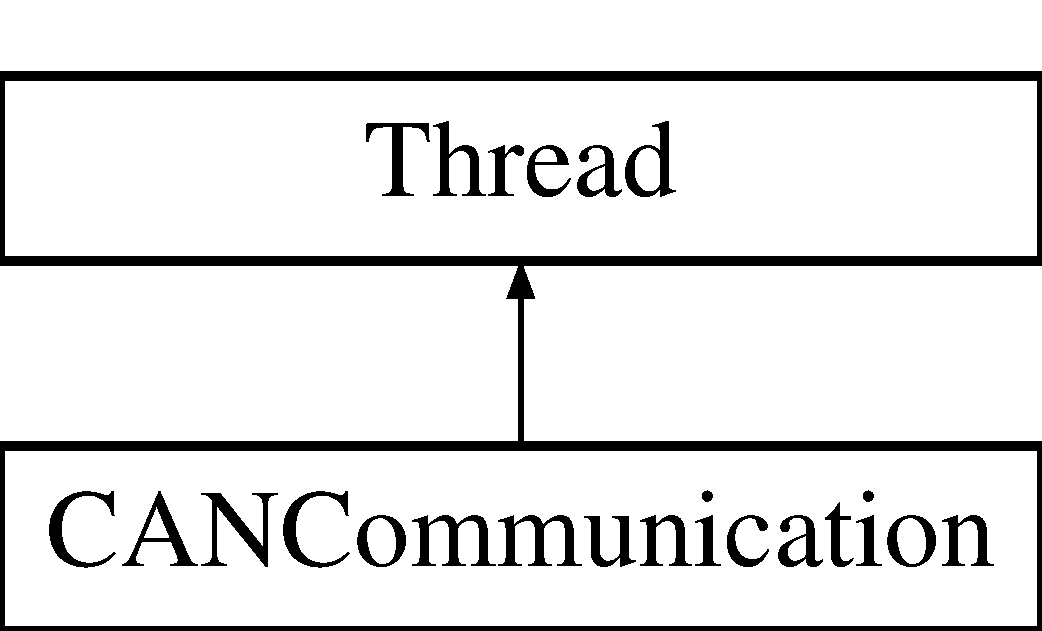
\includegraphics[height=2.000000cm]{class_c_a_n_communication}
\end{center}
\end{figure}
\subsection*{\-Public \-Member \-Functions}
\begin{DoxyCompactItemize}
\item 
\hyperlink{class_c_a_n_communication_ab46dea9c6aacfc3f42361fb458516994}{\-C\-A\-N\-Communication} (bool b\-Dev\-Node\-Given, bool b\-Type\-Given, int n\-Type, \-\_\-\-\_\-u32 dw\-Port, \-\_\-\-\_\-u16 w\-Irq, uint32\-\_\-t bitrate, bool frame\-\_\-extended, string id)
\item 
virtual \hyperlink{class_c_a_n_communication_a1b40a02c0dd8258057d82baf3e8d89be}{$\sim$\-C\-A\-N\-Communication} ()
\item 
virtual bool \hyperlink{class_c_a_n_communication_a548e870616f22b44371eeacac54ec6df}{\-Establish\-Communication} ()
\item 
virtual bool \hyperlink{class_c_a_n_communication_a839851aece22498ef3ab4e807274387b}{\-Configure\-Communication} ()
\item 
bool \hyperlink{class_c_a_n_communication_afb8e85f852dba8f14884b2c988626fed}{\-Close\-Communication} (\-H\-A\-N\-D\-L\-E h)
\item 
virtual bool \hyperlink{class_c_a_n_communication_ada21a063037449022aa654bedb87c522}{\-Send\-Message} (\-T\-P\-C\-A\-N\-Msg $\ast$msg)
\item 
virtual int32\-\_\-t \hyperlink{class_c_a_n_communication_ac3746cec3589757fa7ef73f214801204}{\-Receive\-Message} (\-T\-P\-C\-A\-N\-Rd\-Msg $\ast$msg\-Rx)
\item 
virtual void \hyperlink{class_c_a_n_communication_a8265d49768bb020c101b661b7b36076a}{\-Do\-Work} ()
\item 
void \hyperlink{class_c_a_n_communication_a6221dfb0c7221e7baee07d167ddc2960}{check\-Error\-Write} (int cont\-Write)
\item 
void \hyperlink{class_c_a_n_communication_ac09a44e26ad196ade61428268dee71a0}{check\-Error\-Read} (int cont\-Read)
\end{DoxyCompactItemize}
\subsection*{\-Public \-Attributes}
\begin{DoxyCompactItemize}
\item 
\hypertarget{class_c_a_n_communication_aa2d7f9cb5a7e4e0c1394030dd03d080a}{queue$<$ \-T\-P\-C\-A\-N\-Rd\-Msg $>$ {\bfseries \-Conduccion\-Queue}}\label{class_c_a_n_communication_aa2d7f9cb5a7e4e0c1394030dd03d080a}

\item 
\hypertarget{class_c_a_n_communication_a90482a0006085088e5a8e200abdb39d7}{queue$<$ \-T\-P\-C\-A\-N\-Rd\-Msg $>$ {\bfseries \-Conduccion\-Camion\-Queue}}\label{class_c_a_n_communication_a90482a0006085088e5a8e200abdb39d7}

\item 
\hypertarget{class_c_a_n_communication_a615d966da4be119f6b430c3b4b835433}{pthread\-\_\-mutex\-\_\-t {\bfseries \-Conduccion\-Queue\-\_\-mutex}}\label{class_c_a_n_communication_a615d966da4be119f6b430c3b4b835433}

\item 
\hypertarget{class_c_a_n_communication_a620c2b403b0b88190feb062ce82b3207}{pthread\-\_\-mutex\-\_\-t {\bfseries \-Conduccion\-Camion\-Queue\-\_\-mutex}}\label{class_c_a_n_communication_a620c2b403b0b88190feb062ce82b3207}

\item 
\hypertarget{class_c_a_n_communication_ac3f6acd5a2f05d54d7dde46b41b67ab3}{bool {\bfseries flag\-Active}}\label{class_c_a_n_communication_ac3f6acd5a2f05d54d7dde46b41b67ab3}

\item 
\hypertarget{class_c_a_n_communication_a2ac3e9a2f03766359736929405eb5397}{\hyperlink{class_timer}{\-Timer} {\bfseries \-Communication\-Timer}}\label{class_c_a_n_communication_a2ac3e9a2f03766359736929405eb5397}

\item 
\hypertarget{class_c_a_n_communication_a13abc6674fd555962aa6adf021ffbdf9}{\hyperlink{class_timer}{\-Timer} {\bfseries \-Communication\-Timer2}}\label{class_c_a_n_communication_a13abc6674fd555962aa6adf021ffbdf9}

\item 
\hypertarget{class_c_a_n_communication_a4cd6c441b966fdf076ccb9f82fdc0949}{int {\bfseries cont\-Write}}\label{class_c_a_n_communication_a4cd6c441b966fdf076ccb9f82fdc0949}

\item 
\hypertarget{class_c_a_n_communication_a756857fc938c9b4d549c9a027e7eb6c2}{int {\bfseries cont\-Read}}\label{class_c_a_n_communication_a756857fc938c9b4d549c9a027e7eb6c2}

\item 
\hypertarget{class_c_a_n_communication_ad533c50a8293ca93faa31990b96b1fcd}{bool {\bfseries inicio\-\_\-read\-\_\-write\-\_\-\-C\-A\-N\-\_\-frame}}\label{class_c_a_n_communication_ad533c50a8293ca93faa31990b96b1fcd}

\item 
\hypertarget{class_c_a_n_communication_a5d75d2d21f673a161e902ccbc4821512}{bool {\bfseries error\-Write}}\label{class_c_a_n_communication_a5d75d2d21f673a161e902ccbc4821512}

\item 
\hypertarget{class_c_a_n_communication_ab3b7a5ab3eaa6e45188fb787bf1b60d7}{bool {\bfseries error\-Read}}\label{class_c_a_n_communication_ab3b7a5ab3eaa6e45188fb787bf1b60d7}

\end{DoxyCompactItemize}


\subsection{\-Detailed \-Description}
\-Clase que representa las comunicaciones \-C\-A\-N del subsistema driving. 

\subsection{\-Constructor \& \-Destructor \-Documentation}
\hypertarget{class_c_a_n_communication_ab46dea9c6aacfc3f42361fb458516994}{\index{\-C\-A\-N\-Communication@{\-C\-A\-N\-Communication}!\-C\-A\-N\-Communication@{\-C\-A\-N\-Communication}}
\index{\-C\-A\-N\-Communication@{\-C\-A\-N\-Communication}!CANCommunication@{\-C\-A\-N\-Communication}}
\subsubsection[{\-C\-A\-N\-Communication}]{\setlength{\rightskip}{0pt plus 5cm}{\bf \-C\-A\-N\-Communication\-::\-C\-A\-N\-Communication} (
\begin{DoxyParamCaption}
\item[{bool}]{b\-Dev\-Node\-Given, }
\item[{bool}]{b\-Type\-Given, }
\item[{int}]{n\-Type, }
\item[{\-\_\-\-\_\-u32}]{dw\-Port, }
\item[{\-\_\-\-\_\-u16}]{w\-Irq, }
\item[{uint32\-\_\-t}]{bitrate, }
\item[{bool}]{frame\-\_\-extended, }
\item[{string}]{id}
\end{DoxyParamCaption}
)}}\label{class_c_a_n_communication_ab46dea9c6aacfc3f42361fb458516994}
\-Constructor de la clase 
\begin{DoxyParams}{\-Parameters}
{\em b\-Dev\-Node\-Given} & \-Nodo donde se encuentra definido el puerto en el sistema \\
\hline
{\em b\-Type\-Given} & \-Valor del tipo de nodo \\
\hline
{\em n\-Type} & \-Tipo de dispositivo del \-C\-A\-N \\
\hline
{\em dw\-Port} & \-Puerto en el cual se realiza la conexión \-C\-A\-N \\
\hline
{\em w\-Irq} & \-Configuración \-Irq del dispositivo \-C\-A\-N \\
\hline
{\em bitrate} & \-Velocidad de envío de tramas del \-C\-A\-N \\
\hline
{\em frame\-\_\-extended} & \-Modo de la trama\-: extendida o standart \\
\hline
{\em id} & \-Etiqueta de conexión \\
\hline
\end{DoxyParams}
\hypertarget{class_c_a_n_communication_a1b40a02c0dd8258057d82baf3e8d89be}{\index{\-C\-A\-N\-Communication@{\-C\-A\-N\-Communication}!$\sim$\-C\-A\-N\-Communication@{$\sim$\-C\-A\-N\-Communication}}
\index{$\sim$\-C\-A\-N\-Communication@{$\sim$\-C\-A\-N\-Communication}!CANCommunication@{\-C\-A\-N\-Communication}}
\subsubsection[{$\sim$\-C\-A\-N\-Communication}]{\setlength{\rightskip}{0pt plus 5cm}{\bf \-C\-A\-N\-Communication\-::$\sim$\-C\-A\-N\-Communication} (
\begin{DoxyParamCaption}
{}
\end{DoxyParamCaption}
)\hspace{0.3cm}{\ttfamily  \mbox{[}virtual\mbox{]}}}}\label{class_c_a_n_communication_a1b40a02c0dd8258057d82baf3e8d89be}
\-Destructor de la clase 

\subsection{\-Member \-Function \-Documentation}
\hypertarget{class_c_a_n_communication_ac09a44e26ad196ade61428268dee71a0}{\index{\-C\-A\-N\-Communication@{\-C\-A\-N\-Communication}!check\-Error\-Read@{check\-Error\-Read}}
\index{check\-Error\-Read@{check\-Error\-Read}!CANCommunication@{\-C\-A\-N\-Communication}}
\subsubsection[{check\-Error\-Read}]{\setlength{\rightskip}{0pt plus 5cm}void {\bf \-C\-A\-N\-Communication\-::check\-Error\-Read} (
\begin{DoxyParamCaption}
\item[{int}]{cont\-Read}
\end{DoxyParamCaption}
)}}\label{class_c_a_n_communication_ac09a44e26ad196ade61428268dee71a0}
\-Método que chequea si el numero de tramas de recepción erróneas llegan a un máximo 
\begin{DoxyParams}{\-Parameters}
{\em cont\-Write} & \-Número de tramas de recepción erróneas \\
\hline
\end{DoxyParams}
\hypertarget{class_c_a_n_communication_a6221dfb0c7221e7baee07d167ddc2960}{\index{\-C\-A\-N\-Communication@{\-C\-A\-N\-Communication}!check\-Error\-Write@{check\-Error\-Write}}
\index{check\-Error\-Write@{check\-Error\-Write}!CANCommunication@{\-C\-A\-N\-Communication}}
\subsubsection[{check\-Error\-Write}]{\setlength{\rightskip}{0pt plus 5cm}void {\bf \-C\-A\-N\-Communication\-::check\-Error\-Write} (
\begin{DoxyParamCaption}
\item[{int}]{cont\-Write}
\end{DoxyParamCaption}
)}}\label{class_c_a_n_communication_a6221dfb0c7221e7baee07d167ddc2960}
\-Método que chequea si el numero de tramas de escrituras erróneas llegan a un máximo 
\begin{DoxyParams}{\-Parameters}
{\em cont\-Write} & \-Número de tramas de escrituras erróneas \\
\hline
\end{DoxyParams}
\hypertarget{class_c_a_n_communication_afb8e85f852dba8f14884b2c988626fed}{\index{\-C\-A\-N\-Communication@{\-C\-A\-N\-Communication}!\-Close\-Communication@{\-Close\-Communication}}
\index{\-Close\-Communication@{\-Close\-Communication}!CANCommunication@{\-C\-A\-N\-Communication}}
\subsubsection[{\-Close\-Communication}]{\setlength{\rightskip}{0pt plus 5cm}bool {\bf \-C\-A\-N\-Communication\-::\-Close\-Communication} (
\begin{DoxyParamCaption}
\item[{\-H\-A\-N\-D\-L\-E}]{h}
\end{DoxyParamCaption}
)}}\label{class_c_a_n_communication_afb8e85f852dba8f14884b2c988626fed}
\-Método que configura la conexión \-C\-A\-N \begin{DoxyReturn}{\-Returns}
\-Devuleve si la configuración se ha realizado correctamente 
\end{DoxyReturn}
\hypertarget{class_c_a_n_communication_a839851aece22498ef3ab4e807274387b}{\index{\-C\-A\-N\-Communication@{\-C\-A\-N\-Communication}!\-Configure\-Communication@{\-Configure\-Communication}}
\index{\-Configure\-Communication@{\-Configure\-Communication}!CANCommunication@{\-C\-A\-N\-Communication}}
\subsubsection[{\-Configure\-Communication}]{\setlength{\rightskip}{0pt plus 5cm}bool {\bf \-C\-A\-N\-Communication\-::\-Configure\-Communication} (
\begin{DoxyParamCaption}
{}
\end{DoxyParamCaption}
)\hspace{0.3cm}{\ttfamily  \mbox{[}virtual\mbox{]}}}}\label{class_c_a_n_communication_a839851aece22498ef3ab4e807274387b}
\-Método que configura la conexión \-C\-A\-N \begin{DoxyReturn}{\-Returns}
\-Devuleve si la configuración se ha realizado correctamente 
\end{DoxyReturn}
\hypertarget{class_c_a_n_communication_a8265d49768bb020c101b661b7b36076a}{\index{\-C\-A\-N\-Communication@{\-C\-A\-N\-Communication}!\-Do\-Work@{\-Do\-Work}}
\index{\-Do\-Work@{\-Do\-Work}!CANCommunication@{\-C\-A\-N\-Communication}}
\subsubsection[{\-Do\-Work}]{\setlength{\rightskip}{0pt plus 5cm}void {\bf \-C\-A\-N\-Communication\-::\-Do\-Work} (
\begin{DoxyParamCaption}
{}
\end{DoxyParamCaption}
)\hspace{0.3cm}{\ttfamily  \mbox{[}virtual\mbox{]}}}}\label{class_c_a_n_communication_a8265d49768bb020c101b661b7b36076a}
\-Hilo principal de la clase \hyperlink{class_c_a_n_communication}{\-C\-A\-N\-Communication} que lo que hace es leer mensajes del puerto \-C\-A\-N 

\-Implements \hyperlink{class_thread}{\-Thread}.

\hypertarget{class_c_a_n_communication_a548e870616f22b44371eeacac54ec6df}{\index{\-C\-A\-N\-Communication@{\-C\-A\-N\-Communication}!\-Establish\-Communication@{\-Establish\-Communication}}
\index{\-Establish\-Communication@{\-Establish\-Communication}!CANCommunication@{\-C\-A\-N\-Communication}}
\subsubsection[{\-Establish\-Communication}]{\setlength{\rightskip}{0pt plus 5cm}bool {\bf \-C\-A\-N\-Communication\-::\-Establish\-Communication} (
\begin{DoxyParamCaption}
{}
\end{DoxyParamCaption}
)\hspace{0.3cm}{\ttfamily  \mbox{[}virtual\mbox{]}}}}\label{class_c_a_n_communication_a548e870616f22b44371eeacac54ec6df}
\-Método que establece la comunicación \-C\-A\-N \begin{DoxyReturn}{\-Returns}
\-Devuelve si la conexión se ha establecido correctamente 
\end{DoxyReturn}
\hypertarget{class_c_a_n_communication_ac3746cec3589757fa7ef73f214801204}{\index{\-C\-A\-N\-Communication@{\-C\-A\-N\-Communication}!\-Receive\-Message@{\-Receive\-Message}}
\index{\-Receive\-Message@{\-Receive\-Message}!CANCommunication@{\-C\-A\-N\-Communication}}
\subsubsection[{\-Receive\-Message}]{\setlength{\rightskip}{0pt plus 5cm}int32\-\_\-t {\bf \-C\-A\-N\-Communication\-::\-Receive\-Message} (
\begin{DoxyParamCaption}
\item[{\-T\-P\-C\-A\-N\-Rd\-Msg $\ast$}]{msg\-Rx}
\end{DoxyParamCaption}
)\hspace{0.3cm}{\ttfamily  \mbox{[}virtual\mbox{]}}}}\label{class_c_a_n_communication_ac3746cec3589757fa7ef73f214801204}
\-Método que recive un mensaje \-C\-A\-N 
\begin{DoxyParams}{\-Parameters}
{\em msg\-Tx} & \-Estructura que contiene el mensaje de recepción \-C\-A\-N \\
\hline
\end{DoxyParams}
\begin{DoxyReturn}{\-Returns}
\-Devuelve si el mensaje se ha enviado correctamente 
\end{DoxyReturn}
\hypertarget{class_c_a_n_communication_ada21a063037449022aa654bedb87c522}{\index{\-C\-A\-N\-Communication@{\-C\-A\-N\-Communication}!\-Send\-Message@{\-Send\-Message}}
\index{\-Send\-Message@{\-Send\-Message}!CANCommunication@{\-C\-A\-N\-Communication}}
\subsubsection[{\-Send\-Message}]{\setlength{\rightskip}{0pt plus 5cm}bool {\bf \-C\-A\-N\-Communication\-::\-Send\-Message} (
\begin{DoxyParamCaption}
\item[{\-T\-P\-C\-A\-N\-Msg $\ast$}]{msg\-Tx}
\end{DoxyParamCaption}
)\hspace{0.3cm}{\ttfamily  \mbox{[}virtual\mbox{]}}}}\label{class_c_a_n_communication_ada21a063037449022aa654bedb87c522}
\-Método que envía un mensaje \-C\-A\-N 
\begin{DoxyParams}{\-Parameters}
{\em msg\-Tx} & \-Estructura que contiene el mensaje de envío \-C\-A\-N \\
\hline
\end{DoxyParams}
\begin{DoxyReturn}{\-Returns}
\-Devuelve si el mensaje se ha enviado correctamente 
\end{DoxyReturn}


\-The documentation for this class was generated from the following files\-:\begin{DoxyCompactItemize}
\item 
include/\-Modulo\-\_\-\-Conduccion/\hyperlink{_c_a_n_communication_8hpp}{\-C\-A\-N\-Communication.\-hpp}\item 
src/\hyperlink{_c_a_n_communication_8cpp}{\-C\-A\-N\-Communication.\-cpp}\end{DoxyCompactItemize}

\hypertarget{class_conduccion_thread}{\section{\-Conduccion\-Thread \-Class \-Reference}
\label{class_conduccion_thread}\index{\-Conduccion\-Thread@{\-Conduccion\-Thread}}
}


\-Clase que representa el tratamiento de los menajes \-C\-A\-N que se le envía/recibe el vehículo.  




{\ttfamily \#include $<$\-Conduccion\-Thread.\-hpp$>$}

\-Inheritance diagram for \-Conduccion\-Thread\-:\begin{figure}[H]
\begin{center}
\leavevmode
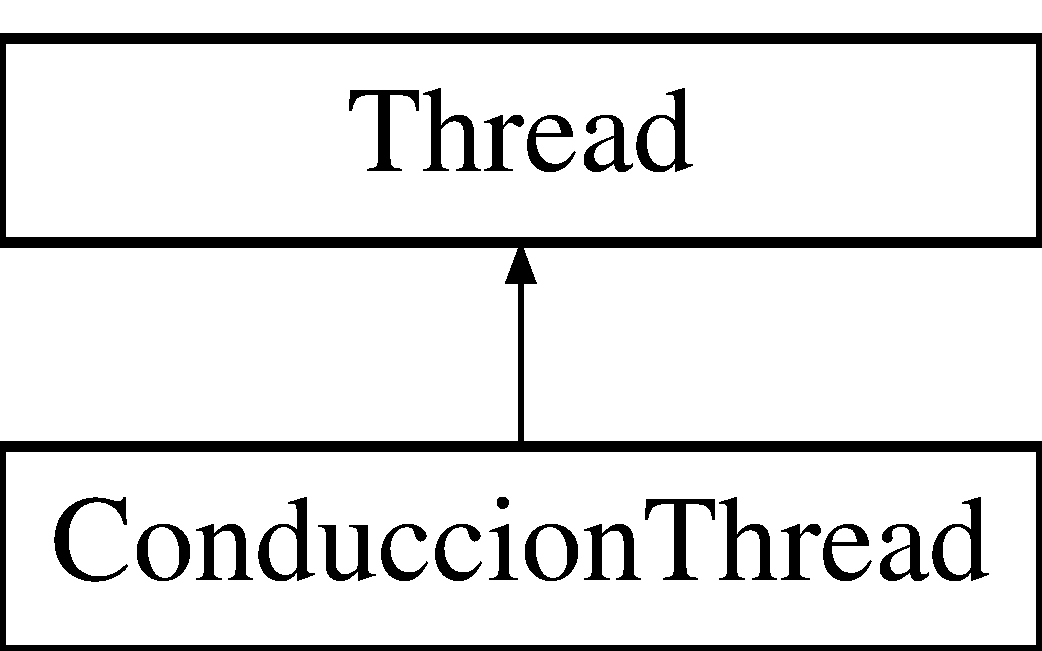
\includegraphics[height=2.000000cm]{class_conduccion_thread}
\end{center}
\end{figure}
\subsection*{\-Public \-Member \-Functions}
\begin{DoxyCompactItemize}
\item 
\hyperlink{class_conduccion_thread_af4208860e61866c8aebd86a58f99f83e}{\-Conduccion\-Thread} (\hyperlink{class_c_a_n_communication}{\-C\-A\-N\-Communication} $\ast$can\-C\-O\-N\-D)
\item 
virtual \hyperlink{class_conduccion_thread_af18549f4e72097c5c82a13975396423a}{$\sim$\-Conduccion\-Thread} ()
\item 
virtual void \hyperlink{class_conduccion_thread_a4267de3c2e18e8b2c3e56cd8e8edfa77}{\-Do\-Work} ()
\item 
void \hyperlink{class_conduccion_thread_ada8b449805f320d94841224eee0cdce5}{m\-\_\-teleop\-\_\-\-C\-A\-N\-\_\-\-A\-U\-T\-O\-M\-A\-T\-A} ()
\item 
void \hyperlink{class_conduccion_thread_a644e33e7220de02cec522de1fa9d3adb}{m\-\_\-engine\-\_\-brake\-\_\-\-C\-A\-N\-\_\-\-A\-U\-T\-O\-M\-A\-T\-A} ()
\item 
void \hyperlink{class_conduccion_thread_ad0a03718e4e843801ff9133763df3020}{m\-\_\-emergency\-\_\-stop\-\_\-\-C\-A\-N\-\_\-\-A\-U\-T\-O\-M\-A\-T\-A} ()
\item 
void \hyperlink{class_conduccion_thread_afa3bfdecad32e8498ed537b01042aff2}{envio\-\_\-trama\-\_\-reinicio\-\_\-\-C\-A\-N\-\_\-\-A\-U\-T\-O\-M\-A\-T\-A} ()
\item 
void \hyperlink{class_conduccion_thread_a291eb5c1d53b449f445db2673d421745}{inicializacion\-\_\-valores\-\_\-tx} ()
\item 
void \hyperlink{class_conduccion_thread_a5a6b4ac4bb02c365951316d4ff881f0c}{m\-\_\-\-Status\-\_\-\-Message\-\_\-\-A\-U\-T\-O\-M\-A\-T\-A\-\_\-\-C\-A\-N} (\-T\-P\-C\-A\-N\-Rd\-Msg \-Status\-Msg)
\item 
void \hyperlink{class_conduccion_thread_abebb162804ed8480b52266fa2e8c1130}{m\-\_\-\-Error\-\_\-\-Message\-\_\-\-A\-U\-T\-O\-M\-A\-T\-A\-\_\-\-C\-A\-N} (\-T\-P\-C\-A\-N\-Rd\-Msg \-Status\-Msg)
\end{DoxyCompactItemize}
\subsection*{\-Public \-Attributes}
\begin{DoxyCompactItemize}
\item 
\hypertarget{class_conduccion_thread_aaed647038c099a0ab408ccef321a2b4a}{pthread\-\_\-mutex\-\_\-t {\bfseries \-Conduccion\-Thread\-\_\-mutex}}\label{class_conduccion_thread_aaed647038c099a0ab408ccef321a2b4a}

\item 
\hypertarget{class_conduccion_thread_a403ef03e71fc3272e4825ce47c23af19}{bool {\bfseries \-C\-O\-N\-D\-U\-C\-C\-I\-O\-N\-\_\-\-A\-C\-T\-I\-V\-E}}\label{class_conduccion_thread_a403ef03e71fc3272e4825ce47c23af19}

\item 
\hypertarget{class_conduccion_thread_aa31ebdd2a99392133312f5f55388cbb2}{bool {\bfseries flag\-\_\-active\-\_\-backup}}\label{class_conduccion_thread_aa31ebdd2a99392133312f5f55388cbb2}

\item 
\hypertarget{class_conduccion_thread_ac267a2a1bef42087301ac8bf1d80cdaa}{short {\bfseries valor\-\_\-arranque\-\_\-parada}}\label{class_conduccion_thread_ac267a2a1bef42087301ac8bf1d80cdaa}

\item 
\hypertarget{class_conduccion_thread_a027aac83ca25ec528c272026bdba4744}{short {\bfseries valor\-\_\-freno\-\_\-estacionamiento}}\label{class_conduccion_thread_a027aac83ca25ec528c272026bdba4744}

\item 
\hypertarget{class_conduccion_thread_af522b2c32ac9be0c3f3cbdd90011912c}{short {\bfseries acelerador\-\_\-tx}}\label{class_conduccion_thread_af522b2c32ac9be0c3f3cbdd90011912c}

\item 
\hypertarget{class_conduccion_thread_a7fa33669ea495a7279d47b370e7318ac}{short {\bfseries velocidad\-\_\-tx}}\label{class_conduccion_thread_a7fa33669ea495a7279d47b370e7318ac}

\item 
\hypertarget{class_conduccion_thread_a7f7f4e74587782e5ee4820fc3e10ef69}{short {\bfseries freno\-\_\-servicio\-\_\-tx}}\label{class_conduccion_thread_a7f7f4e74587782e5ee4820fc3e10ef69}

\item 
\hypertarget{class_conduccion_thread_a53c06f8afb12b02c90161cf79bee3832}{short {\bfseries valor\-\_\-marcha}}\label{class_conduccion_thread_a53c06f8afb12b02c90161cf79bee3832}

\item 
\hypertarget{class_conduccion_thread_af5d168172fb768c1faf1d1b169a35bbb}{short {\bfseries cambio\-\_\-marcha\-\_\-tx}}\label{class_conduccion_thread_af5d168172fb768c1faf1d1b169a35bbb}

\item 
\hypertarget{class_conduccion_thread_afb7dea488a424dde8dd3b14cc1fd6762}{short {\bfseries sentido\-\_\-direccion\-\_\-tx}}\label{class_conduccion_thread_afb7dea488a424dde8dd3b14cc1fd6762}

\item 
\hypertarget{class_conduccion_thread_a0b2410e2414a60cdf4f3d23a5ea6324e}{short {\bfseries direccion\-\_\-tx}}\label{class_conduccion_thread_a0b2410e2414a60cdf4f3d23a5ea6324e}

\item 
\hypertarget{class_conduccion_thread_a357ae9530e53f77b49e061a1efc110d5}{short {\bfseries valor\-\_\-direccion}}\label{class_conduccion_thread_a357ae9530e53f77b49e061a1efc110d5}

\item 
\hypertarget{class_conduccion_thread_a9acb1cfde19437bf396aa3efe44e1081}{short {\bfseries valor\-\_\-luces}}\label{class_conduccion_thread_a9acb1cfde19437bf396aa3efe44e1081}

\item 
\hypertarget{class_conduccion_thread_acd7791ecaa072c4a439a28e9d1b6f4e5}{short {\bfseries valor\-\_\-luces\-\_\-\-I\-R}}\label{class_conduccion_thread_acd7791ecaa072c4a439a28e9d1b6f4e5}

\item 
\hypertarget{class_conduccion_thread_a9851b5f9c6ad1f9c8d71498b6081d290}{short {\bfseries valor\-\_\-diferencial}}\label{class_conduccion_thread_a9851b5f9c6ad1f9c8d71498b6081d290}

\item 
\hypertarget{class_conduccion_thread_aee22628f727ee2a33224bc6010a4443d}{short {\bfseries valor\-\_\-laser}}\label{class_conduccion_thread_aee22628f727ee2a33224bc6010a4443d}

\item 
\hypertarget{class_conduccion_thread_a2371b144beb68d9a86f9025dddf6d8ba}{short {\bfseries valor\-\_\-parada\-\_\-emergencia}}\label{class_conduccion_thread_a2371b144beb68d9a86f9025dddf6d8ba}

\item 
\hypertarget{class_conduccion_thread_a051c3cfaa09dc000627cf45b2e520a4c}{uint8\-\_\-t {\bfseries byte\-\_\-7}}\label{class_conduccion_thread_a051c3cfaa09dc000627cf45b2e520a4c}

\item 
\hypertarget{class_conduccion_thread_acf1873ccee4ce10dac23017aa7b6c3ad}{short {\bfseries arranque\-\_\-parada}}\label{class_conduccion_thread_acf1873ccee4ce10dac23017aa7b6c3ad}

\item 
\hypertarget{class_conduccion_thread_ac78c299549691cca4b12fdc5a330ef16}{short {\bfseries freno\-\_\-estacionamiento}}\label{class_conduccion_thread_ac78c299549691cca4b12fdc5a330ef16}

\item 
\hypertarget{class_conduccion_thread_a52209657e37aeb8416654702a689fdd9}{short {\bfseries conmutador\-\_\-m\-\_\-a}}\label{class_conduccion_thread_a52209657e37aeb8416654702a689fdd9}

\item 
\hypertarget{class_conduccion_thread_a580a948849a18a610b7a13a3017bcb91}{short {\bfseries acelerador}}\label{class_conduccion_thread_a580a948849a18a610b7a13a3017bcb91}

\item 
\hypertarget{class_conduccion_thread_af2b3c6b9f1d12885115905124f183f1f}{short {\bfseries velocidad}}\label{class_conduccion_thread_af2b3c6b9f1d12885115905124f183f1f}

\item 
\hypertarget{class_conduccion_thread_a79f043e0c8a1f4e1af6059ae751a7e00}{short {\bfseries freno\-\_\-servicio}}\label{class_conduccion_thread_a79f043e0c8a1f4e1af6059ae751a7e00}

\item 
\hypertarget{class_conduccion_thread_ac8a3034d0d7fb45dac02833dfa7671b7}{short {\bfseries marcha\-\_\-actual}}\label{class_conduccion_thread_ac8a3034d0d7fb45dac02833dfa7671b7}

\item 
\hypertarget{class_conduccion_thread_a272f1aba8ef25f8d2e5f1b18839f5e84}{short {\bfseries sentido\-\_\-marcha}}\label{class_conduccion_thread_a272f1aba8ef25f8d2e5f1b18839f5e84}

\item 
\hypertarget{class_conduccion_thread_a490a54758fc10174c3296c1bc8a8818a}{short {\bfseries direccion}}\label{class_conduccion_thread_a490a54758fc10174c3296c1bc8a8818a}

\item 
\hypertarget{class_conduccion_thread_a309acc3f3239bf03aed0d09cc5f5e9ac}{short {\bfseries conf\-\_\-parada\-\_\-emergencia}}\label{class_conduccion_thread_a309acc3f3239bf03aed0d09cc5f5e9ac}

\item 
\hypertarget{class_conduccion_thread_afdeb8f2fe8ac2aac12739546e66e034c}{short {\bfseries parada\-\_\-emergencia\-\_\-obstaculo}}\label{class_conduccion_thread_afdeb8f2fe8ac2aac12739546e66e034c}

\item 
\hypertarget{class_conduccion_thread_a8582bb8005611928ee7adad13e392ea5}{short {\bfseries parada\-\_\-emergencia\-\_\-remota}}\label{class_conduccion_thread_a8582bb8005611928ee7adad13e392ea5}

\item 
\hypertarget{class_conduccion_thread_a2e71fa8b1e2fda996e60a7fad26f9453}{short {\bfseries parada\-\_\-emergencia\-\_\-local}}\label{class_conduccion_thread_a2e71fa8b1e2fda996e60a7fad26f9453}

\item 
\hypertarget{class_conduccion_thread_a29f4159aa0ea8d5d5e51e973cfca9166}{short {\bfseries error\-\_\-arranque\-\_\-parada}}\label{class_conduccion_thread_a29f4159aa0ea8d5d5e51e973cfca9166}

\item 
\hypertarget{class_conduccion_thread_a5b9bc034347928a7ada5b59f5449795b}{short {\bfseries error\-\_\-acelerador}}\label{class_conduccion_thread_a5b9bc034347928a7ada5b59f5449795b}

\item 
\hypertarget{class_conduccion_thread_a9da8e5de08c1962e0776c1dd459aae6f}{short {\bfseries error\-\_\-freno\-\_\-estacionamiento}}\label{class_conduccion_thread_a9da8e5de08c1962e0776c1dd459aae6f}

\item 
\hypertarget{class_conduccion_thread_a66e012a6849293985a7cdd5d95803ce6}{short {\bfseries error\-\_\-freno\-\_\-servicio}}\label{class_conduccion_thread_a66e012a6849293985a7cdd5d95803ce6}

\item 
\hypertarget{class_conduccion_thread_ac4909c2ae76a41854d65d7bdef69c47e}{short {\bfseries error\-\_\-cambio\-\_\-marcha}}\label{class_conduccion_thread_ac4909c2ae76a41854d65d7bdef69c47e}

\item 
\hypertarget{class_conduccion_thread_a8261f17b8cd5d13adc5275e16733cc44}{short {\bfseries error\-\_\-direccion}}\label{class_conduccion_thread_a8261f17b8cd5d13adc5275e16733cc44}

\item 
\hypertarget{class_conduccion_thread_a13bae73eda9adf8544e105c8c6d85467}{short {\bfseries error\-\_\-bloqueo\-\_\-diferenciales}}\label{class_conduccion_thread_a13bae73eda9adf8544e105c8c6d85467}

\item 
\hypertarget{class_conduccion_thread_ae64f68126af967e86cf46620486bf961}{bool {\bfseries parada\-Emergencia}}\label{class_conduccion_thread_ae64f68126af967e86cf46620486bf961}

\item 
\hypertarget{class_conduccion_thread_a29640b1b31c6ca5d85e7640284e4bbf7}{int {\bfseries tipo\-\_\-parada}}\label{class_conduccion_thread_a29640b1b31c6ca5d85e7640284e4bbf7}

\item 
\hypertarget{class_conduccion_thread_a56fb420f61e01a9a98c397f95abdab7c}{int {\bfseries tipo\-\_\-parada\-\_\-emergencia}}\label{class_conduccion_thread_a56fb420f61e01a9a98c397f95abdab7c}

\item 
\hypertarget{class_conduccion_thread_aac780ac9687c7f507c919a748399654e}{\hyperlink{class_timer}{\-Timer} {\bfseries t}}\label{class_conduccion_thread_aac780ac9687c7f507c919a748399654e}

\end{DoxyCompactItemize}


\subsection{\-Detailed \-Description}
\-Clase que representa el tratamiento de los menajes \-C\-A\-N que se le envía/recibe el vehículo. 

\subsection{\-Constructor \& \-Destructor \-Documentation}
\hypertarget{class_conduccion_thread_af4208860e61866c8aebd86a58f99f83e}{\index{\-Conduccion\-Thread@{\-Conduccion\-Thread}!\-Conduccion\-Thread@{\-Conduccion\-Thread}}
\index{\-Conduccion\-Thread@{\-Conduccion\-Thread}!ConduccionThread@{\-Conduccion\-Thread}}
\subsubsection[{\-Conduccion\-Thread}]{\setlength{\rightskip}{0pt plus 5cm}{\bf \-Conduccion\-Thread\-::\-Conduccion\-Thread} (
\begin{DoxyParamCaption}
\item[{{\bf \-C\-A\-N\-Communication} $\ast$}]{can\-C\-O\-N\-D}
\end{DoxyParamCaption}
)}}\label{class_conduccion_thread_af4208860e61866c8aebd86a58f99f83e}
\-Constructor de la clase \hyperlink{class_conduccion_thread}{\-Conduccion\-Thread} 
\begin{DoxyParams}{\-Parameters}
{\em can\-C\-O\-N\-D} & \-Variable que contiene un objeto de la clase \hyperlink{class_c_a_n_communication}{\-C\-A\-N\-Communication} \\
\hline
\end{DoxyParams}
\hypertarget{class_conduccion_thread_af18549f4e72097c5c82a13975396423a}{\index{\-Conduccion\-Thread@{\-Conduccion\-Thread}!$\sim$\-Conduccion\-Thread@{$\sim$\-Conduccion\-Thread}}
\index{$\sim$\-Conduccion\-Thread@{$\sim$\-Conduccion\-Thread}!ConduccionThread@{\-Conduccion\-Thread}}
\subsubsection[{$\sim$\-Conduccion\-Thread}]{\setlength{\rightskip}{0pt plus 5cm}{\bf \-Conduccion\-Thread\-::$\sim$\-Conduccion\-Thread} (
\begin{DoxyParamCaption}
{}
\end{DoxyParamCaption}
)\hspace{0.3cm}{\ttfamily  \mbox{[}virtual\mbox{]}}}}\label{class_conduccion_thread_af18549f4e72097c5c82a13975396423a}
\-Destructor de la clase \hyperlink{class_conduccion_thread}{\-Conduccion\-Thread} 

\subsection{\-Member \-Function \-Documentation}
\hypertarget{class_conduccion_thread_a4267de3c2e18e8b2c3e56cd8e8edfa77}{\index{\-Conduccion\-Thread@{\-Conduccion\-Thread}!\-Do\-Work@{\-Do\-Work}}
\index{\-Do\-Work@{\-Do\-Work}!ConduccionThread@{\-Conduccion\-Thread}}
\subsubsection[{\-Do\-Work}]{\setlength{\rightskip}{0pt plus 5cm}void {\bf \-Conduccion\-Thread\-::\-Do\-Work} (
\begin{DoxyParamCaption}
{}
\end{DoxyParamCaption}
)\hspace{0.3cm}{\ttfamily  \mbox{[}virtual\mbox{]}}}}\label{class_conduccion_thread_a4267de3c2e18e8b2c3e56cd8e8edfa77}
\-Hilo de la clase \hyperlink{class_conduccion_thread}{\-Conduccion\-Thread} que se encarga de desencolar los mensajes de una pila para su posterior tratamiento 

\-Implements \hyperlink{class_thread}{\-Thread}.

\hypertarget{class_conduccion_thread_afa3bfdecad32e8498ed537b01042aff2}{\index{\-Conduccion\-Thread@{\-Conduccion\-Thread}!envio\-\_\-trama\-\_\-reinicio\-\_\-\-C\-A\-N\-\_\-\-A\-U\-T\-O\-M\-A\-T\-A@{envio\-\_\-trama\-\_\-reinicio\-\_\-\-C\-A\-N\-\_\-\-A\-U\-T\-O\-M\-A\-T\-A}}
\index{envio\-\_\-trama\-\_\-reinicio\-\_\-\-C\-A\-N\-\_\-\-A\-U\-T\-O\-M\-A\-T\-A@{envio\-\_\-trama\-\_\-reinicio\-\_\-\-C\-A\-N\-\_\-\-A\-U\-T\-O\-M\-A\-T\-A}!ConduccionThread@{\-Conduccion\-Thread}}
\subsubsection[{envio\-\_\-trama\-\_\-reinicio\-\_\-\-C\-A\-N\-\_\-\-A\-U\-T\-O\-M\-A\-T\-A}]{\setlength{\rightskip}{0pt plus 5cm}void {\bf \-Conduccion\-Thread\-::envio\-\_\-trama\-\_\-reinicio\-\_\-\-C\-A\-N\-\_\-\-A\-U\-T\-O\-M\-A\-T\-A} (
\begin{DoxyParamCaption}
{}
\end{DoxyParamCaption}
)}}\label{class_conduccion_thread_afa3bfdecad32e8498ed537b01042aff2}
\-Método que envía un mensaje al vehículo con el reinicio de todas las variables que afectan al funcionamiento del vehículo \hypertarget{class_conduccion_thread_a291eb5c1d53b449f445db2673d421745}{\index{\-Conduccion\-Thread@{\-Conduccion\-Thread}!inicializacion\-\_\-valores\-\_\-tx@{inicializacion\-\_\-valores\-\_\-tx}}
\index{inicializacion\-\_\-valores\-\_\-tx@{inicializacion\-\_\-valores\-\_\-tx}!ConduccionThread@{\-Conduccion\-Thread}}
\subsubsection[{inicializacion\-\_\-valores\-\_\-tx}]{\setlength{\rightskip}{0pt plus 5cm}void {\bf \-Conduccion\-Thread\-::inicializacion\-\_\-valores\-\_\-tx} (
\begin{DoxyParamCaption}
{}
\end{DoxyParamCaption}
)}}\label{class_conduccion_thread_a291eb5c1d53b449f445db2673d421745}
\-Método que realiza una inicialización de los valores de la clase \hyperlink{class_conduccion_thread}{\-Conduccion\-Thread} \hypertarget{class_conduccion_thread_ad0a03718e4e843801ff9133763df3020}{\index{\-Conduccion\-Thread@{\-Conduccion\-Thread}!m\-\_\-emergency\-\_\-stop\-\_\-\-C\-A\-N\-\_\-\-A\-U\-T\-O\-M\-A\-T\-A@{m\-\_\-emergency\-\_\-stop\-\_\-\-C\-A\-N\-\_\-\-A\-U\-T\-O\-M\-A\-T\-A}}
\index{m\-\_\-emergency\-\_\-stop\-\_\-\-C\-A\-N\-\_\-\-A\-U\-T\-O\-M\-A\-T\-A@{m\-\_\-emergency\-\_\-stop\-\_\-\-C\-A\-N\-\_\-\-A\-U\-T\-O\-M\-A\-T\-A}!ConduccionThread@{\-Conduccion\-Thread}}
\subsubsection[{m\-\_\-emergency\-\_\-stop\-\_\-\-C\-A\-N\-\_\-\-A\-U\-T\-O\-M\-A\-T\-A}]{\setlength{\rightskip}{0pt plus 5cm}void {\bf \-Conduccion\-Thread\-::m\-\_\-emergency\-\_\-stop\-\_\-\-C\-A\-N\-\_\-\-A\-U\-T\-O\-M\-A\-T\-A} (
\begin{DoxyParamCaption}
{}
\end{DoxyParamCaption}
)}}\label{class_conduccion_thread_ad0a03718e4e843801ff9133763df3020}
\-Método que envía un mensaje al vehículo para que realice una parada de emergencía \hypertarget{class_conduccion_thread_a644e33e7220de02cec522de1fa9d3adb}{\index{\-Conduccion\-Thread@{\-Conduccion\-Thread}!m\-\_\-engine\-\_\-brake\-\_\-\-C\-A\-N\-\_\-\-A\-U\-T\-O\-M\-A\-T\-A@{m\-\_\-engine\-\_\-brake\-\_\-\-C\-A\-N\-\_\-\-A\-U\-T\-O\-M\-A\-T\-A}}
\index{m\-\_\-engine\-\_\-brake\-\_\-\-C\-A\-N\-\_\-\-A\-U\-T\-O\-M\-A\-T\-A@{m\-\_\-engine\-\_\-brake\-\_\-\-C\-A\-N\-\_\-\-A\-U\-T\-O\-M\-A\-T\-A}!ConduccionThread@{\-Conduccion\-Thread}}
\subsubsection[{m\-\_\-engine\-\_\-brake\-\_\-\-C\-A\-N\-\_\-\-A\-U\-T\-O\-M\-A\-T\-A}]{\setlength{\rightskip}{0pt plus 5cm}void {\bf \-Conduccion\-Thread\-::m\-\_\-engine\-\_\-brake\-\_\-\-C\-A\-N\-\_\-\-A\-U\-T\-O\-M\-A\-T\-A} (
\begin{DoxyParamCaption}
{}
\end{DoxyParamCaption}
)}}\label{class_conduccion_thread_a644e33e7220de02cec522de1fa9d3adb}
\-Método que envía un mensaje con la puesta del freno de mano y con el vehículo parado \hypertarget{class_conduccion_thread_abebb162804ed8480b52266fa2e8c1130}{\index{\-Conduccion\-Thread@{\-Conduccion\-Thread}!m\-\_\-\-Error\-\_\-\-Message\-\_\-\-A\-U\-T\-O\-M\-A\-T\-A\-\_\-\-C\-A\-N@{m\-\_\-\-Error\-\_\-\-Message\-\_\-\-A\-U\-T\-O\-M\-A\-T\-A\-\_\-\-C\-A\-N}}
\index{m\-\_\-\-Error\-\_\-\-Message\-\_\-\-A\-U\-T\-O\-M\-A\-T\-A\-\_\-\-C\-A\-N@{m\-\_\-\-Error\-\_\-\-Message\-\_\-\-A\-U\-T\-O\-M\-A\-T\-A\-\_\-\-C\-A\-N}!ConduccionThread@{\-Conduccion\-Thread}}
\subsubsection[{m\-\_\-\-Error\-\_\-\-Message\-\_\-\-A\-U\-T\-O\-M\-A\-T\-A\-\_\-\-C\-A\-N}]{\setlength{\rightskip}{0pt plus 5cm}void {\bf \-Conduccion\-Thread\-::m\-\_\-\-Error\-\_\-\-Message\-\_\-\-A\-U\-T\-O\-M\-A\-T\-A\-\_\-\-C\-A\-N} (
\begin{DoxyParamCaption}
\item[{\-T\-P\-C\-A\-N\-Rd\-Msg}]{\-Status\-Msg}
\end{DoxyParamCaption}
)}}\label{class_conduccion_thread_abebb162804ed8480b52266fa2e8c1130}
\-Método que gestiona los mensajes de error que llegan del autómata 
\begin{DoxyParams}{\-Parameters}
{\em \-Status\-Msg} & \-Variable que contiene mensajes \-C\-A\-N con los posibles errores que haya en el autómata \\
\hline
\end{DoxyParams}
\hypertarget{class_conduccion_thread_a5a6b4ac4bb02c365951316d4ff881f0c}{\index{\-Conduccion\-Thread@{\-Conduccion\-Thread}!m\-\_\-\-Status\-\_\-\-Message\-\_\-\-A\-U\-T\-O\-M\-A\-T\-A\-\_\-\-C\-A\-N@{m\-\_\-\-Status\-\_\-\-Message\-\_\-\-A\-U\-T\-O\-M\-A\-T\-A\-\_\-\-C\-A\-N}}
\index{m\-\_\-\-Status\-\_\-\-Message\-\_\-\-A\-U\-T\-O\-M\-A\-T\-A\-\_\-\-C\-A\-N@{m\-\_\-\-Status\-\_\-\-Message\-\_\-\-A\-U\-T\-O\-M\-A\-T\-A\-\_\-\-C\-A\-N}!ConduccionThread@{\-Conduccion\-Thread}}
\subsubsection[{m\-\_\-\-Status\-\_\-\-Message\-\_\-\-A\-U\-T\-O\-M\-A\-T\-A\-\_\-\-C\-A\-N}]{\setlength{\rightskip}{0pt plus 5cm}void {\bf \-Conduccion\-Thread\-::m\-\_\-\-Status\-\_\-\-Message\-\_\-\-A\-U\-T\-O\-M\-A\-T\-A\-\_\-\-C\-A\-N} (
\begin{DoxyParamCaption}
\item[{\-T\-P\-C\-A\-N\-Rd\-Msg}]{\-Status\-Msg}
\end{DoxyParamCaption}
)}}\label{class_conduccion_thread_a5a6b4ac4bb02c365951316d4ff881f0c}
\-Método que realiza el tratamiento de los mensajes enviados al autómata 
\begin{DoxyParams}{\-Parameters}
{\em \-Status\-Msg} & \-Variable que contiene una estructura con el mensaje que se envíara al autómata \\
\hline
\end{DoxyParams}
\hypertarget{class_conduccion_thread_ada8b449805f320d94841224eee0cdce5}{\index{\-Conduccion\-Thread@{\-Conduccion\-Thread}!m\-\_\-teleop\-\_\-\-C\-A\-N\-\_\-\-A\-U\-T\-O\-M\-A\-T\-A@{m\-\_\-teleop\-\_\-\-C\-A\-N\-\_\-\-A\-U\-T\-O\-M\-A\-T\-A}}
\index{m\-\_\-teleop\-\_\-\-C\-A\-N\-\_\-\-A\-U\-T\-O\-M\-A\-T\-A@{m\-\_\-teleop\-\_\-\-C\-A\-N\-\_\-\-A\-U\-T\-O\-M\-A\-T\-A}!ConduccionThread@{\-Conduccion\-Thread}}
\subsubsection[{m\-\_\-teleop\-\_\-\-C\-A\-N\-\_\-\-A\-U\-T\-O\-M\-A\-T\-A}]{\setlength{\rightskip}{0pt plus 5cm}void {\bf \-Conduccion\-Thread\-::m\-\_\-teleop\-\_\-\-C\-A\-N\-\_\-\-A\-U\-T\-O\-M\-A\-T\-A} (
\begin{DoxyParamCaption}
{}
\end{DoxyParamCaption}
)}}\label{class_conduccion_thread_ada8b449805f320d94841224eee0cdce5}
\-Método que gestiona el envío de mensajes \-C\-A\-N al autómata 

\-The documentation for this class was generated from the following files\-:\begin{DoxyCompactItemize}
\item 
include/\-Modulo\-\_\-\-Conduccion/\hyperlink{_conduccion_thread_8hpp}{\-Conduccion\-Thread.\-hpp}\item 
src/\hyperlink{_conduccion_thread_8cpp}{\-Conduccion\-Thread.\-cpp}\end{DoxyCompactItemize}

\hypertarget{class_thread}{\section{\-Thread \-Class \-Reference}
\label{class_thread}\index{\-Thread@{\-Thread}}
}


\-Clase que representa el hilo de ejecución a través del cual se van a escribir/leer mensajes \-C\-A\-N para luego procesarlos.  




{\ttfamily \#include $<$\-Thread.\-hpp$>$}

\-Inheritance diagram for \-Thread\-:\begin{figure}[H]
\begin{center}
\leavevmode
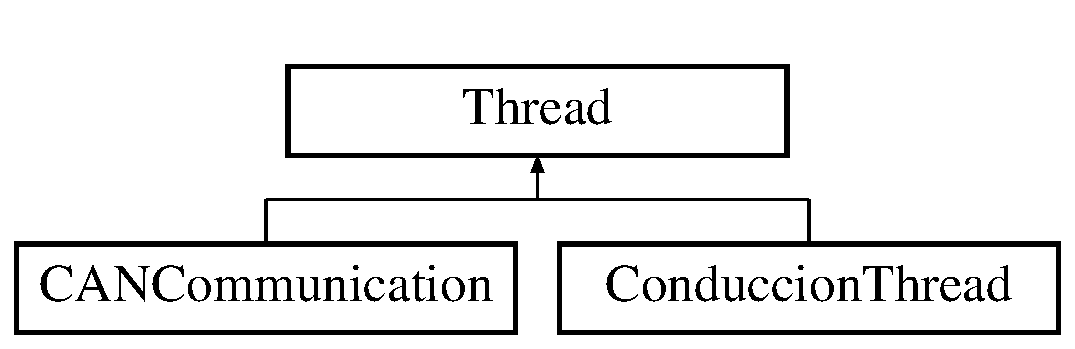
\includegraphics[height=2.000000cm]{class_thread}
\end{center}
\end{figure}
\subsection*{\-Public \-Member \-Functions}
\begin{DoxyCompactItemize}
\item 
virtual \hyperlink{class_thread_a37d9edd3a1a776cbc27dedff949c9726}{$\sim$\-Thread} ()
\item 
void \hyperlink{class_thread_a26c650bc1d2d290979a2f693569ab9c8}{\-Run} ()  throw (\-Thread\-Exception)
\item 
void \hyperlink{class_thread_a9a7979cfd00ccef6276a2ea47ed5a464}{\-Terminate} ()  throw (\-Thread\-Exception)
\item 
bool \hyperlink{class_thread_add375d7ae010c2297c01154b3cb84d32}{\-Is\-Active} ()
\end{DoxyCompactItemize}
\subsection*{\-Public \-Attributes}
\begin{DoxyCompactItemize}
\item 
\hypertarget{class_thread_a33f1a9a1e8b8797bb0ca17059f1c4dbc}{pthread\-\_\-t {\bfseries handler}}\label{class_thread_a33f1a9a1e8b8797bb0ca17059f1c4dbc}

\end{DoxyCompactItemize}
\subsection*{\-Protected \-Member \-Functions}
\begin{DoxyCompactItemize}
\item 
\hypertarget{class_thread_a7db4848a0eebac704a82048e11e97c0f}{virtual void {\bfseries \-Do\-Work} ()=0}\label{class_thread_a7db4848a0eebac704a82048e11e97c0f}

\end{DoxyCompactItemize}
\subsection*{\-Protected \-Attributes}
\begin{DoxyCompactItemize}
\item 
\hypertarget{class_thread_aead2efd9497d0a22b184eb9056a82fdf}{bool {\bfseries active}}\label{class_thread_aead2efd9497d0a22b184eb9056a82fdf}

\end{DoxyCompactItemize}


\subsection{\-Detailed \-Description}
\-Clase que representa el hilo de ejecución a través del cual se van a escribir/leer mensajes \-C\-A\-N para luego procesarlos. 

\subsection{\-Constructor \& \-Destructor \-Documentation}
\hypertarget{class_thread_a37d9edd3a1a776cbc27dedff949c9726}{\index{\-Thread@{\-Thread}!$\sim$\-Thread@{$\sim$\-Thread}}
\index{$\sim$\-Thread@{$\sim$\-Thread}!Thread@{\-Thread}}
\subsubsection[{$\sim$\-Thread}]{\setlength{\rightskip}{0pt plus 5cm}{\bf \-Thread\-::$\sim$\-Thread} (
\begin{DoxyParamCaption}
{}
\end{DoxyParamCaption}
)\hspace{0.3cm}{\ttfamily  \mbox{[}virtual\mbox{]}}}}\label{class_thread_a37d9edd3a1a776cbc27dedff949c9726}
\-Destructor de la clase 

\subsection{\-Member \-Function \-Documentation}
\hypertarget{class_thread_add375d7ae010c2297c01154b3cb84d32}{\index{\-Thread@{\-Thread}!\-Is\-Active@{\-Is\-Active}}
\index{\-Is\-Active@{\-Is\-Active}!Thread@{\-Thread}}
\subsubsection[{\-Is\-Active}]{\setlength{\rightskip}{0pt plus 5cm}bool {\bf \-Thread\-::\-Is\-Active} (
\begin{DoxyParamCaption}
{}
\end{DoxyParamCaption}
)}}\label{class_thread_add375d7ae010c2297c01154b3cb84d32}
\-Método que indica si el hilo de ejecución está activo \begin{DoxyReturn}{\-Returns}
\-Devuelve si el hilo está activo 
\end{DoxyReturn}
\hypertarget{class_thread_a26c650bc1d2d290979a2f693569ab9c8}{\index{\-Thread@{\-Thread}!\-Run@{\-Run}}
\index{\-Run@{\-Run}!Thread@{\-Thread}}
\subsubsection[{\-Run}]{\setlength{\rightskip}{0pt plus 5cm}void {\bf \-Thread\-::\-Run} (
\begin{DoxyParamCaption}
{}
\end{DoxyParamCaption}
)  throw ({\bf \-Thread\-Exception})}}\label{class_thread_a26c650bc1d2d290979a2f693569ab9c8}
\-Método que hace correr el hilo de ejecución \hypertarget{class_thread_a9a7979cfd00ccef6276a2ea47ed5a464}{\index{\-Thread@{\-Thread}!\-Terminate@{\-Terminate}}
\index{\-Terminate@{\-Terminate}!Thread@{\-Thread}}
\subsubsection[{\-Terminate}]{\setlength{\rightskip}{0pt plus 5cm}void {\bf \-Thread\-::\-Terminate} (
\begin{DoxyParamCaption}
{}
\end{DoxyParamCaption}
)  throw ({\bf \-Thread\-Exception})}}\label{class_thread_a9a7979cfd00ccef6276a2ea47ed5a464}
\-Método que hace terminar el hilo de ejecución 

\-The documentation for this class was generated from the following files\-:\begin{DoxyCompactItemize}
\item 
include/\-Modulo\-\_\-\-Conduccion/\hyperlink{_thread_8hpp}{\-Thread.\-hpp}\item 
src/\hyperlink{_thread_8cpp}{\-Thread.\-cpp}\end{DoxyCompactItemize}

\hypertarget{class_thread_exception}{\section{\-Thread\-Exception \-Class \-Reference}
\label{class_thread_exception}\index{\-Thread\-Exception@{\-Thread\-Exception}}
}


\-Clase que representa un mensaje de excepción por si la ejecución del hilo diera un errror.  




{\ttfamily \#include $<$\-Thread.\-hpp$>$}

\subsection*{\-Public \-Member \-Functions}
\begin{DoxyCompactItemize}
\item 
\hyperlink{class_thread_exception_a3effcc3da05430c4b7700cd7cd1345e3}{\-Thread\-Exception} (const string \&message, bool incl\-Sys\-Msg=false)  throw ()
\item 
\hyperlink{class_thread_exception_a4c09e4a9676f90c25d9581f5235666d4}{$\sim$\-Thread\-Exception} ()  throw ()
\item 
const char $\ast$ \hyperlink{class_thread_exception_aaf731aac495bf3711f229e53c4fcb04b}{what} () const   throw ()
\end{DoxyCompactItemize}


\subsection{\-Detailed \-Description}
\-Clase que representa un mensaje de excepción por si la ejecución del hilo diera un errror. 

\subsection{\-Constructor \& \-Destructor \-Documentation}
\hypertarget{class_thread_exception_a3effcc3da05430c4b7700cd7cd1345e3}{\index{\-Thread\-Exception@{\-Thread\-Exception}!\-Thread\-Exception@{\-Thread\-Exception}}
\index{\-Thread\-Exception@{\-Thread\-Exception}!ThreadException@{\-Thread\-Exception}}
\subsubsection[{\-Thread\-Exception}]{\setlength{\rightskip}{0pt plus 5cm}{\bf \-Thread\-Exception\-::\-Thread\-Exception} (
\begin{DoxyParamCaption}
\item[{const string \&}]{message, }
\item[{bool}]{incl\-Sys\-Msg = {\ttfamily false}}
\end{DoxyParamCaption}
)  throw ()}}\label{class_thread_exception_a3effcc3da05430c4b7700cd7cd1345e3}
\-Constructor de la clase \hyperlink{class_thread_exception}{\-Thread\-Exception} 
\begin{DoxyParams}{\-Parameters}
{\em message} & \-Mensaje de error que aparacería si hubiera una excepción \\
\hline
{\em incl\-Sys\-Msg} & \-Variable que indica si se ha producido un error \\
\hline
\end{DoxyParams}
\hypertarget{class_thread_exception_a4c09e4a9676f90c25d9581f5235666d4}{\index{\-Thread\-Exception@{\-Thread\-Exception}!$\sim$\-Thread\-Exception@{$\sim$\-Thread\-Exception}}
\index{$\sim$\-Thread\-Exception@{$\sim$\-Thread\-Exception}!ThreadException@{\-Thread\-Exception}}
\subsubsection[{$\sim$\-Thread\-Exception}]{\setlength{\rightskip}{0pt plus 5cm}{\bf \-Thread\-Exception\-::$\sim$\-Thread\-Exception} (
\begin{DoxyParamCaption}
{}
\end{DoxyParamCaption}
)  throw ()}}\label{class_thread_exception_a4c09e4a9676f90c25d9581f5235666d4}
\-Método que lanza la excepcion 

\subsection{\-Member \-Function \-Documentation}
\hypertarget{class_thread_exception_aaf731aac495bf3711f229e53c4fcb04b}{\index{\-Thread\-Exception@{\-Thread\-Exception}!what@{what}}
\index{what@{what}!ThreadException@{\-Thread\-Exception}}
\subsubsection[{what}]{\setlength{\rightskip}{0pt plus 5cm}const char $\ast$ {\bf \-Thread\-Exception\-::what} (
\begin{DoxyParamCaption}
{}
\end{DoxyParamCaption}
) const  throw ()}}\label{class_thread_exception_aaf731aac495bf3711f229e53c4fcb04b}
\-Método que devuelve el mensaje de excepción \begin{DoxyReturn}{\-Returns}
\-Devuelve el mensaje de excepción 
\end{DoxyReturn}


\-The documentation for this class was generated from the following files\-:\begin{DoxyCompactItemize}
\item 
include/\-Modulo\-\_\-\-Conduccion/\hyperlink{_thread_8hpp}{\-Thread.\-hpp}\item 
src/\hyperlink{_thread_8cpp}{\-Thread.\-cpp}\end{DoxyCompactItemize}

\hypertarget{class_timer}{\section{\-Timer \-Class \-Reference}
\label{class_timer}\index{\-Timer@{\-Timer}}
}


\-Clase que representa un temporizador utilizado para contear la frecuencia de de publicación del nodo \-R\-O\-S.  




{\ttfamily \#include $<$\-Timer.\-hpp$>$}

\subsection*{\-Public \-Member \-Functions}
\begin{DoxyCompactItemize}
\item 
\hyperlink{class_timer_a5f16e8da27d2a5a5242dead46de05d97}{\-Timer} ()
\item 
void \hyperlink{class_timer_ae7c0c1e7d12de4b8a6e7c64e451cdd2a}{\-Reset} ()
\item 
double \hyperlink{class_timer_af1ec46b36eb5b90f7b4dfad29f9aee5b}{\-Get\-Timed} ()
\item 
float \hyperlink{class_timer_a3bb0f087deb92ce89270ebe5f5adbf13}{\-Get\-Time} ()
\item 
int \hyperlink{class_timer_a9f907e1cf928fcbe790b16490cc50a7b}{\-Get\-State} ()
\item 
void \hyperlink{class_timer_a75556dc66dcca80ebd21e6e460d24219}{\-Enable} ()
\item 
void \hyperlink{class_timer_a90fe39d8a55ad3b9d662d227109a588c}{\-Disable} ()
\item 
void \hyperlink{class_timer_a4c33d0dbe892a1ad8c784cbf043b3b26}{\-Wait\-Until} (double t)
\item 
void \hyperlink{class_timer_ac77f20e91f884c90b89021fb448909ea}{\-Wait\-Until} (float t)
\end{DoxyCompactItemize}
\subsection*{\-Public \-Attributes}
\begin{DoxyCompactItemize}
\item 
\hypertarget{class_timer_a2d6d1eddef72b6c3680265003cb1bf9a}{int {\bfseries state}}\label{class_timer_a2d6d1eddef72b6c3680265003cb1bf9a}

\end{DoxyCompactItemize}


\subsection{\-Detailed \-Description}
\-Clase que representa un temporizador utilizado para contear la frecuencia de de publicación del nodo \-R\-O\-S. 

\subsection{\-Constructor \& \-Destructor \-Documentation}
\hypertarget{class_timer_a5f16e8da27d2a5a5242dead46de05d97}{\index{\-Timer@{\-Timer}!\-Timer@{\-Timer}}
\index{\-Timer@{\-Timer}!Timer@{\-Timer}}
\subsubsection[{\-Timer}]{\setlength{\rightskip}{0pt plus 5cm}{\bf \-Timer\-::\-Timer} (
\begin{DoxyParamCaption}
{}
\end{DoxyParamCaption}
)}}\label{class_timer_a5f16e8da27d2a5a5242dead46de05d97}
\-Constructor de la clase 

\subsection{\-Member \-Function \-Documentation}
\hypertarget{class_timer_a90fe39d8a55ad3b9d662d227109a588c}{\index{\-Timer@{\-Timer}!\-Disable@{\-Disable}}
\index{\-Disable@{\-Disable}!Timer@{\-Timer}}
\subsubsection[{\-Disable}]{\setlength{\rightskip}{0pt plus 5cm}void {\bf \-Timer\-::\-Disable} (
\begin{DoxyParamCaption}
{}
\end{DoxyParamCaption}
)}}\label{class_timer_a90fe39d8a55ad3b9d662d227109a588c}
\-Método público que deshabilita el temporizador e inicia la cuenta \hypertarget{class_timer_a75556dc66dcca80ebd21e6e460d24219}{\index{\-Timer@{\-Timer}!\-Enable@{\-Enable}}
\index{\-Enable@{\-Enable}!Timer@{\-Timer}}
\subsubsection[{\-Enable}]{\setlength{\rightskip}{0pt plus 5cm}void {\bf \-Timer\-::\-Enable} (
\begin{DoxyParamCaption}
{}
\end{DoxyParamCaption}
)}}\label{class_timer_a75556dc66dcca80ebd21e6e460d24219}
\-Método público que habilita el temporizador e inicia la cuenta \hypertarget{class_timer_a9f907e1cf928fcbe790b16490cc50a7b}{\index{\-Timer@{\-Timer}!\-Get\-State@{\-Get\-State}}
\index{\-Get\-State@{\-Get\-State}!Timer@{\-Timer}}
\subsubsection[{\-Get\-State}]{\setlength{\rightskip}{0pt plus 5cm}int {\bf \-Timer\-::\-Get\-State} (
\begin{DoxyParamCaption}
{}
\end{DoxyParamCaption}
)}}\label{class_timer_a9f907e1cf928fcbe790b16490cc50a7b}
\-Método público que devuelde el estado del \hyperlink{class_timer}{\-Timer} \begin{DoxyReturn}{\-Returns}
\-Estado del timer 
\end{DoxyReturn}
\hypertarget{class_timer_a3bb0f087deb92ce89270ebe5f5adbf13}{\index{\-Timer@{\-Timer}!\-Get\-Time@{\-Get\-Time}}
\index{\-Get\-Time@{\-Get\-Time}!Timer@{\-Timer}}
\subsubsection[{\-Get\-Time}]{\setlength{\rightskip}{0pt plus 5cm}float {\bf \-Timer\-::\-Get\-Time} (
\begin{DoxyParamCaption}
{}
\end{DoxyParamCaption}
)}}\label{class_timer_a3bb0f087deb92ce89270ebe5f5adbf13}
\-Método público que obtiene los segundos desde la inicialización del temporizador \begin{DoxyReturn}{\-Returns}
\-Número de segundos desde la inicialización del temporizador en un formato específico 
\end{DoxyReturn}
\hypertarget{class_timer_af1ec46b36eb5b90f7b4dfad29f9aee5b}{\index{\-Timer@{\-Timer}!\-Get\-Timed@{\-Get\-Timed}}
\index{\-Get\-Timed@{\-Get\-Timed}!Timer@{\-Timer}}
\subsubsection[{\-Get\-Timed}]{\setlength{\rightskip}{0pt plus 5cm}double {\bf \-Timer\-::\-Get\-Timed} (
\begin{DoxyParamCaption}
{}
\end{DoxyParamCaption}
)}}\label{class_timer_af1ec46b36eb5b90f7b4dfad29f9aee5b}
\-Método público que obtiene los segundos desde la inicialización del temporizador \begin{DoxyReturn}{\-Returns}
\-Número de segundos desde la inicialización del temporizador 
\end{DoxyReturn}
\hypertarget{class_timer_ae7c0c1e7d12de4b8a6e7c64e451cdd2a}{\index{\-Timer@{\-Timer}!\-Reset@{\-Reset}}
\index{\-Reset@{\-Reset}!Timer@{\-Timer}}
\subsubsection[{\-Reset}]{\setlength{\rightskip}{0pt plus 5cm}void {\bf \-Timer\-::\-Reset} (
\begin{DoxyParamCaption}
{}
\end{DoxyParamCaption}
)}}\label{class_timer_ae7c0c1e7d12de4b8a6e7c64e451cdd2a}
\-Método público que efectúa un reinicio de la cuenta del temportizador \hypertarget{class_timer_a4c33d0dbe892a1ad8c784cbf043b3b26}{\index{\-Timer@{\-Timer}!\-Wait\-Until@{\-Wait\-Until}}
\index{\-Wait\-Until@{\-Wait\-Until}!Timer@{\-Timer}}
\subsubsection[{\-Wait\-Until}]{\setlength{\rightskip}{0pt plus 5cm}void {\bf \-Timer\-::\-Wait\-Until} (
\begin{DoxyParamCaption}
\item[{double}]{t}
\end{DoxyParamCaption}
)}}\label{class_timer_a4c33d0dbe892a1ad8c784cbf043b3b26}
\-Método público que realiza una espera 
\begin{DoxyParams}{\-Parameters}
{\em \-Número} & de segundos a realizar la espera \\
\hline
\end{DoxyParams}
\hypertarget{class_timer_ac77f20e91f884c90b89021fb448909ea}{\index{\-Timer@{\-Timer}!\-Wait\-Until@{\-Wait\-Until}}
\index{\-Wait\-Until@{\-Wait\-Until}!Timer@{\-Timer}}
\subsubsection[{\-Wait\-Until}]{\setlength{\rightskip}{0pt plus 5cm}void {\bf \-Timer\-::\-Wait\-Until} (
\begin{DoxyParamCaption}
\item[{float}]{t}
\end{DoxyParamCaption}
)}}\label{class_timer_ac77f20e91f884c90b89021fb448909ea}
\-Método público que realiza una espera 
\begin{DoxyParams}{\-Parameters}
{\em \-Número} & de segundos a realizar la espera \\
\hline
\end{DoxyParams}


\-The documentation for this class was generated from the following files\-:\begin{DoxyCompactItemize}
\item 
include/\-Modulo\-\_\-\-Conduccion/\hyperlink{_timer_8hpp}{\-Timer.\-hpp}\item 
src/\hyperlink{_timer_8cpp}{\-Timer.\-cpp}\end{DoxyCompactItemize}

\chapter{\-File \-Documentation}
\hypertarget{_c_a_n_communication_8hpp}{\section{include/\-Modulo\-\_\-\-Conduccion/\-C\-A\-N\-Communication.hpp \-File \-Reference}
\label{_c_a_n_communication_8hpp}\index{include/\-Modulo\-\_\-\-Conduccion/\-C\-A\-N\-Communication.\-hpp@{include/\-Modulo\-\_\-\-Conduccion/\-C\-A\-N\-Communication.\-hpp}}
}


\-Declara el tipo de la clase \char`\"{}\-C\-A\-N\-Communication\char`\"{}.  


{\ttfamily \#include $<$libpcan.\-h$>$}\*
{\ttfamily \#include $<$queue$>$}\*
{\ttfamily \#include $<$errno.\-h$>$}\*
{\ttfamily \#include $<$unistd.\-h$>$}\*
{\ttfamily \#include $<$signal.\-h$>$}\*
{\ttfamily \#include $<$stdio.\-h$>$}\*
{\ttfamily \#include $<$string$>$}\*
{\ttfamily \#include $<$iostream$>$}\*
{\ttfamily \#include $<$stdlib.\-h$>$}\*
{\ttfamily \#include $<$sstream$>$}\*
{\ttfamily \#include $<$fcntl.\-h$>$}\*
{\ttfamily \#include $<$stdint.\-h$>$}\*
{\ttfamily \#include \char`\"{}\-Thread.\-hpp\char`\"{}}\*
{\ttfamily \#include \char`\"{}\-Timer.\-hpp\char`\"{}}\*
\subsection*{\-Classes}
\begin{DoxyCompactItemize}
\item 
class \hyperlink{class_c_a_n_communication}{\-C\-A\-N\-Communication}
\begin{DoxyCompactList}\small\item\em \-Clase que representa las comunicaciones \-C\-A\-N del subsistema driving. \end{DoxyCompactList}\end{DoxyCompactItemize}
\subsection*{\-Defines}
\begin{DoxyCompactItemize}
\item 
\hypertarget{_c_a_n_communication_8hpp_a7ce36d8e87af0db87c0d228a64201e35}{\#define \hyperlink{_c_a_n_communication_8hpp_a7ce36d8e87af0db87c0d228a64201e35}{\-D\-E\-F\-A\-U\-L\-T\-\_\-\-N\-O\-D\-E}~\char`\"{}/dev/pcan0\char`\"{}}\label{_c_a_n_communication_8hpp_a7ce36d8e87af0db87c0d228a64201e35}

\begin{DoxyCompactList}\small\item\em \-Nombre del nodo en el que conectado el dispositivo \-C\-A\-N. \end{DoxyCompactList}\item 
\hypertarget{_c_a_n_communication_8hpp_aa088cea88928bbb5cafe1b935db2f11b}{\#define \hyperlink{_c_a_n_communication_8hpp_aa088cea88928bbb5cafe1b935db2f11b}{\-E\-R\-R\-O\-R\-\_\-\-W\-R\-I\-T\-E\-\_\-\-F\-R\-A\-M\-E}~1000}\label{_c_a_n_communication_8hpp_aa088cea88928bbb5cafe1b935db2f11b}

\begin{DoxyCompactList}\small\item\em \-Número de tramas de escrituras erroneas a partir de las cuales saltaria un error de escritura. \end{DoxyCompactList}\item 
\hypertarget{_c_a_n_communication_8hpp_a03f698b2bab6a81653418f32fc4a62b0}{\#define \hyperlink{_c_a_n_communication_8hpp_a03f698b2bab6a81653418f32fc4a62b0}{\-E\-R\-R\-O\-R\-\_\-\-R\-E\-A\-D\-\_\-\-F\-R\-A\-M\-E}~1000}\label{_c_a_n_communication_8hpp_a03f698b2bab6a81653418f32fc4a62b0}

\begin{DoxyCompactList}\small\item\em \-Número de tramas de lectura erroneas a partir de las cuales saltaria un error de lectura. \end{DoxyCompactList}\end{DoxyCompactItemize}


\subsection{\-Detailed \-Description}
\-Declara el tipo de la clase \char`\"{}\-C\-A\-N\-Communication\char`\"{}. 
\begin{DoxyItemize}
\item \-La clase implementa la escritura/lectura de los mensajes \-C\-A\-N del \-Subsistema \-Driving \begin{DoxyAuthor}{\-Author}
\-Sergio \-Doctor 
\end{DoxyAuthor}
\begin{DoxyDate}{\-Date}
2014 
\end{DoxyDate}

\end{DoxyItemize}
\hypertarget{_conduccion_thread_8hpp}{\section{include/\-Modulo\-\_\-\-Conduccion/\-Conduccion\-Thread.hpp \-File \-Reference}
\label{_conduccion_thread_8hpp}\index{include/\-Modulo\-\_\-\-Conduccion/\-Conduccion\-Thread.\-hpp@{include/\-Modulo\-\_\-\-Conduccion/\-Conduccion\-Thread.\-hpp}}
}


\-Declara el tipo de la clase \char`\"{}\-Conduccion\-Thread\char`\"{}.  


{\ttfamily \#include \char`\"{}\-Thread.\-hpp\char`\"{}}\*
{\ttfamily \#include \char`\"{}\-C\-A\-N\-Communication.\-hpp\char`\"{}}\*
{\ttfamily \#include \char`\"{}\-Timer.\-hpp\char`\"{}}\*
{\ttfamily \#include $<$queue$>$}\*
\subsection*{\-Classes}
\begin{DoxyCompactItemize}
\item 
class \hyperlink{class_conduccion_thread}{\-Conduccion\-Thread}
\begin{DoxyCompactList}\small\item\em \-Clase que representa el tratamiento de los menajes \-C\-A\-N que se le envía/recibe el vehículo. \end{DoxyCompactList}\end{DoxyCompactItemize}
\subsection*{\-Defines}
\begin{DoxyCompactItemize}
\item 
\hypertarget{_conduccion_thread_8hpp_a9cf883931e4ebfe282a433d2b54b760c}{\#define \hyperlink{_conduccion_thread_8hpp_a9cf883931e4ebfe282a433d2b54b760c}{\-A\-R\-R\-A\-N\-Q\-U\-E\-\_\-\-P\-A\-R\-A\-D\-A}~0x01}\label{_conduccion_thread_8hpp_a9cf883931e4ebfe282a433d2b54b760c}

\begin{DoxyCompactList}\small\item\em \-Valor del arranque del vehículo // \-En binario (0000 0001) \end{DoxyCompactList}\item 
\hypertarget{_conduccion_thread_8hpp_ac1425cbe6a6055717e08b62984924a7d}{\#define \hyperlink{_conduccion_thread_8hpp_ac1425cbe6a6055717e08b62984924a7d}{\-F\-R\-E\-N\-O\-\_\-\-E\-S\-T\-A\-C\-I\-O\-N\-A\-M\-I\-E\-N\-T\-O}~0x02}\label{_conduccion_thread_8hpp_ac1425cbe6a6055717e08b62984924a7d}

\begin{DoxyCompactList}\small\item\em \-Valor del freno de estacionamiento // \-En binario (0000 0010) \end{DoxyCompactList}\item 
\hypertarget{_conduccion_thread_8hpp_accc898f427bcfab8f8554d0683a736de}{\#define \hyperlink{_conduccion_thread_8hpp_accc898f427bcfab8f8554d0683a736de}{\-M\-A\-N}~0x00}\label{_conduccion_thread_8hpp_accc898f427bcfab8f8554d0683a736de}

\begin{DoxyCompactList}\small\item\em \-Valor del freno de estacionamiento // \-En binario (0000 0000) \end{DoxyCompactList}\item 
\hypertarget{_conduccion_thread_8hpp_a0cc6f7717df9fbdc0f33efb88720a639}{\#define \hyperlink{_conduccion_thread_8hpp_a0cc6f7717df9fbdc0f33efb88720a639}{\-A\-U\-T\-O}~0x01}\label{_conduccion_thread_8hpp_a0cc6f7717df9fbdc0f33efb88720a639}

\begin{DoxyCompactList}\small\item\em \-Valor del freno de estacionamiento // \-En binario (0000 0001) \end{DoxyCompactList}\item 
\hypertarget{_conduccion_thread_8hpp_ab92b0d3f26ea0fd591739e3942414a5d}{\#define \hyperlink{_conduccion_thread_8hpp_ab92b0d3f26ea0fd591739e3942414a5d}{\-M\-A\-R\-C\-H\-A\-\_\-\-H\-\_\-}~0x08}\label{_conduccion_thread_8hpp_ab92b0d3f26ea0fd591739e3942414a5d}

\begin{DoxyCompactList}\small\item\em \-Valor de la \-Marcha \-H // \-En binario (0000 1000) \end{DoxyCompactList}\item 
\hypertarget{_conduccion_thread_8hpp_afdb9f1f9f6931227fd35364484ef7452}{\#define \hyperlink{_conduccion_thread_8hpp_afdb9f1f9f6931227fd35364484ef7452}{\-M\-A\-R\-C\-H\-A\-\_\-\-N\-\_\-}~0x10}\label{_conduccion_thread_8hpp_afdb9f1f9f6931227fd35364484ef7452}

\begin{DoxyCompactList}\small\item\em \-Valor de la \-Marcha \-N // \-En binario (0001 0000) \end{DoxyCompactList}\item 
\hypertarget{_conduccion_thread_8hpp_ac96f50ae847e8acb6f8f37d18cc6c224}{\#define \hyperlink{_conduccion_thread_8hpp_ac96f50ae847e8acb6f8f37d18cc6c224}{\-M\-A\-R\-C\-H\-A\-\_\-\-R\-\_\-}~0x20}\label{_conduccion_thread_8hpp_ac96f50ae847e8acb6f8f37d18cc6c224}

\begin{DoxyCompactList}\small\item\em \-Valor de la \-Marcha \-R // \-En binario (0010 0000) \end{DoxyCompactList}\item 
\hypertarget{_conduccion_thread_8hpp_a2b066b1c9420c785e88330d573a4f3c1}{\#define \hyperlink{_conduccion_thread_8hpp_a2b066b1c9420c785e88330d573a4f3c1}{\-M\-A\-R\-C\-H\-A\-\_\-\-N1\-\_\-}~0x40}\label{_conduccion_thread_8hpp_a2b066b1c9420c785e88330d573a4f3c1}

\begin{DoxyCompactList}\small\item\em \-Valor de la \-Marcha \-N1 // \-En binario (0100 0000) \end{DoxyCompactList}\item 
\hypertarget{_conduccion_thread_8hpp_abb4bf703c0c62fb12284617022f1e85b}{\#define \hyperlink{_conduccion_thread_8hpp_abb4bf703c0c62fb12284617022f1e85b}{\-M\-A\-R\-C\-H\-A\-\_\-\-L\-\_\-}~0x80}\label{_conduccion_thread_8hpp_abb4bf703c0c62fb12284617022f1e85b}

\begin{DoxyCompactList}\small\item\em \-Valor de la \-Marcha \-L // \-En binario (1000 0000) \end{DoxyCompactList}\item 
\hypertarget{_conduccion_thread_8hpp_aad0115ce280fb4af2b295eb2fe59754d}{\#define \hyperlink{_conduccion_thread_8hpp_aad0115ce280fb4af2b295eb2fe59754d}{\-C\-O\-N\-F\-\_\-\-P\-A\-R\-A\-D\-A\-\_\-\-E\-M\-E\-R\-G\-E\-N\-C\-I\-A}~0x01}\label{_conduccion_thread_8hpp_aad0115ce280fb4af2b295eb2fe59754d}

\begin{DoxyCompactList}\small\item\em \-Valor de la confirmación de la parada de emergencia // \-En binario (0000 0001) \end{DoxyCompactList}\item 
\hypertarget{_conduccion_thread_8hpp_a9946b019c8818a6a2d138a0142f8aafb}{\#define \hyperlink{_conduccion_thread_8hpp_a9946b019c8818a6a2d138a0142f8aafb}{\-P\-A\-R\-A\-D\-A\-\_\-\-E\-M\-E\-R\-G\-E\-N\-C\-I\-A\-\_\-\-O\-B\-S\-T\-A\-C\-U\-L\-O}~0x02}\label{_conduccion_thread_8hpp_a9946b019c8818a6a2d138a0142f8aafb}

\begin{DoxyCompactList}\small\item\em \-Valor de la señal de activación/desactivación del láser // \-En binario (0000 0010) -\/$>$$>$$>$$>$ \-Señal de activación/desactivacion del laser. \end{DoxyCompactList}\item 
\hypertarget{_conduccion_thread_8hpp_aa96d36caa33bde05fc2a0bc1040e0ffa}{\#define \hyperlink{_conduccion_thread_8hpp_aa96d36caa33bde05fc2a0bc1040e0ffa}{\-P\-A\-R\-A\-D\-A\-\_\-\-E\-M\-E\-R\-G\-E\-N\-C\-I\-A\-\_\-\-R\-E\-M\-O\-T\-A}~0x04}\label{_conduccion_thread_8hpp_aa96d36caa33bde05fc2a0bc1040e0ffa}

\begin{DoxyCompactList}\small\item\em \-Valor de la señal de parada por activación de la seta remota // \-En binario (0000 0100) -\/$>$$>$$>$$>$ \-Señal de parada por la seta remota. \end{DoxyCompactList}\item 
\hypertarget{_conduccion_thread_8hpp_a75d4392df15c1b2b1d2475284a42677d}{\#define \hyperlink{_conduccion_thread_8hpp_a75d4392df15c1b2b1d2475284a42677d}{\-P\-A\-R\-A\-D\-A\-\_\-\-E\-M\-E\-R\-G\-E\-N\-C\-I\-A\-\_\-\-L\-O\-C\-A\-L}~0x08}\label{_conduccion_thread_8hpp_a75d4392df15c1b2b1d2475284a42677d}

\begin{DoxyCompactList}\small\item\em \-Valor de la señal de parada por activación de la seta del vehículo // \-En binario (0000 1000) -\/$>$$>$$>$$>$ \-Señal de parada por la seta del vehiculo. \end{DoxyCompactList}\end{DoxyCompactItemize}


\subsection{\-Detailed \-Description}
\-Declara el tipo de la clase \char`\"{}\-Conduccion\-Thread\char`\"{}. \-Implementación del main principal del \-Subsistema \-Driving.


\begin{DoxyItemize}
\item \-La clase implementa el tratamiento de los mensajes \-C\-A\-N que se reciben/envían del \-Subsistema \-Driving \begin{DoxyAuthor}{\-Author}
\-Sergio \-Doctor 
\end{DoxyAuthor}
\begin{DoxyDate}{\-Date}
2014
\end{DoxyDate}
\begin{DoxyAuthor}{\-Author}
\-Sergio \-Doctor 
\end{DoxyAuthor}
\begin{DoxyDate}{\-Date}
2014 
\end{DoxyDate}

\end{DoxyItemize}
\hypertarget{interaction_8h}{\section{include/\-Modulo\-\_\-\-Conduccion/interaction.h \-File \-Reference}
\label{interaction_8h}\index{include/\-Modulo\-\_\-\-Conduccion/interaction.\-h@{include/\-Modulo\-\_\-\-Conduccion/interaction.\-h}}
}


\-Archivo de cabecera de \hyperlink{interaction_8cpp}{interaction.\-cpp}.  


{\ttfamily \#include $<$stdlib.\-h$>$}\*
{\ttfamily \#include $<$iostream$>$}\*
\subsection*{\-Functions}
\begin{DoxyCompactItemize}
\item 
int \hyperlink{interaction_8h_a94c6e54f2ff017b3027c7727d82f87db}{get\-Operation\-Mode} (int, char $\ast$$\ast$)
\item 
void \hyperlink{interaction_8h_aea6fd7b41b6bd83bfa7f24353403ea66}{print\-Correct\-Syntax} ()
\end{DoxyCompactItemize}


\subsection{\-Detailed \-Description}
\-Archivo de cabecera de \hyperlink{interaction_8cpp}{interaction.\-cpp}. \begin{DoxyAuthor}{\-Author}
\-Carlos \-Amores 
\end{DoxyAuthor}
\begin{DoxyDate}{\-Date}
10/03/2014 
\end{DoxyDate}


\subsection{\-Function \-Documentation}
\hypertarget{interaction_8h_a94c6e54f2ff017b3027c7727d82f87db}{\index{interaction.\-h@{interaction.\-h}!get\-Operation\-Mode@{get\-Operation\-Mode}}
\index{get\-Operation\-Mode@{get\-Operation\-Mode}!interaction.h@{interaction.\-h}}
\subsubsection[{get\-Operation\-Mode}]{\setlength{\rightskip}{0pt plus 5cm}int {\bf get\-Operation\-Mode} (
\begin{DoxyParamCaption}
\item[{int}]{argc, }
\item[{char $\ast$$\ast$}]{argv}
\end{DoxyParamCaption}
)}}\label{interaction_8h_a94c6e54f2ff017b3027c7727d82f87db}
\-Función principal que elige una versión del software dependiendo del argumento de entrada 
\begin{DoxyParams}[1]{\-Parameters}
\mbox{\tt in}  & {\em argc} & \-Número de argumentos \\
\hline
\mbox{\tt in}  & {\em argv} & \-Vector de argumentos \\
\hline
\end{DoxyParams}
\begin{DoxyReturn}{\-Returns}
\-Devuelve 0 si hay errores o número de versión si no hay errores 
\end{DoxyReturn}
\hypertarget{interaction_8h_aea6fd7b41b6bd83bfa7f24353403ea66}{\index{interaction.\-h@{interaction.\-h}!print\-Correct\-Syntax@{print\-Correct\-Syntax}}
\index{print\-Correct\-Syntax@{print\-Correct\-Syntax}!interaction.h@{interaction.\-h}}
\subsubsection[{print\-Correct\-Syntax}]{\setlength{\rightskip}{0pt plus 5cm}void {\bf print\-Correct\-Syntax} (
\begin{DoxyParamCaption}
{}
\end{DoxyParamCaption}
)}}\label{interaction_8h_aea6fd7b41b6bd83bfa7f24353403ea66}
\-Muestra por pantalla que se ha producido un error al elegir versión. \-Presenta la manera de ejecutar el programa correctamente 
\hypertarget{_thread_8hpp}{\section{include/\-Modulo\-\_\-\-Conduccion/\-Thread.hpp \-File \-Reference}
\label{_thread_8hpp}\index{include/\-Modulo\-\_\-\-Conduccion/\-Thread.\-hpp@{include/\-Modulo\-\_\-\-Conduccion/\-Thread.\-hpp}}
}


\-Declara el tipo de la clase \char`\"{}\-Thread\char`\"{}.  


{\ttfamily \#include $<$pthread.\-h$>$}\*
{\ttfamily \#include $<$errno.\-h$>$}\*
{\ttfamily \#include $<$string.\-h$>$}\*
{\ttfamily \#include $<$exception$>$}\*
{\ttfamily \#include $<$string$>$}\*
\subsection*{\-Classes}
\begin{DoxyCompactItemize}
\item 
class \hyperlink{class_thread_exception}{\-Thread\-Exception}
\begin{DoxyCompactList}\small\item\em \-Clase que representa un mensaje de excepción por si la ejecución del hilo diera un errror. \end{DoxyCompactList}\item 
class \hyperlink{class_thread}{\-Thread}
\begin{DoxyCompactList}\small\item\em \-Clase que representa el hilo de ejecución a través del cual se van a escribir/leer mensajes \-C\-A\-N para luego procesarlos. \end{DoxyCompactList}\end{DoxyCompactItemize}


\subsection{\-Detailed \-Description}
\-Declara el tipo de la clase \char`\"{}\-Thread\char`\"{}. 
\begin{DoxyItemize}
\item \-La clase implementa el hilo de ejecución de la clase \hyperlink{class_c_a_n_communication}{\-C\-A\-N\-Communication} \begin{DoxyAuthor}{\-Author}
\-Sergio \-Doctor 
\end{DoxyAuthor}
\begin{DoxyDate}{\-Date}
2014 
\end{DoxyDate}

\end{DoxyItemize}
\hypertarget{_timer_8hpp}{\section{include/\-Modulo\-\_\-\-Conduccion/\-Timer.hpp \-File \-Reference}
\label{_timer_8hpp}\index{include/\-Modulo\-\_\-\-Conduccion/\-Timer.\-hpp@{include/\-Modulo\-\_\-\-Conduccion/\-Timer.\-hpp}}
}


\-Declara el tipo de la clase \char`\"{}\-Timer\char`\"{}.  


\subsection*{\-Classes}
\begin{DoxyCompactItemize}
\item 
class \hyperlink{class_timer}{\-Timer}
\begin{DoxyCompactList}\small\item\em \-Clase que representa un temporizador utilizado para contear la frecuencia de de publicación del nodo \-R\-O\-S. \end{DoxyCompactList}\end{DoxyCompactItemize}
\subsection*{\-Functions}
\begin{DoxyCompactItemize}
\item 
\hypertarget{namespace_time_a9a5a6e05c93a85b0d298e7c75052255f}{void {\bfseries \-Time\-::\-Wait} (double t)}\label{namespace_time_a9a5a6e05c93a85b0d298e7c75052255f}

\item 
\hypertarget{namespace_time_afc4402c7a9fed2825de20bf54191ec48}{void {\bfseries \-Time\-::\-Wait} (float t)}\label{namespace_time_afc4402c7a9fed2825de20bf54191ec48}

\item 
\hypertarget{namespace_time_a150759388a1a8e6b261dd833a9f9eca0}{double {\bfseries \-Time\-::\-Timed} ()}\label{namespace_time_a150759388a1a8e6b261dd833a9f9eca0}

\item 
\hypertarget{namespace_time_abe79148949d6a5217eebde6563089d06}{float {\bfseries \-Time\-::\-Time} ()}\label{namespace_time_abe79148949d6a5217eebde6563089d06}

\end{DoxyCompactItemize}


\subsection{\-Detailed \-Description}
\-Declara el tipo de la clase \char`\"{}\-Timer\char`\"{}. 
\begin{DoxyItemize}
\item \-La clase implementa la gestión de un temporizador \begin{DoxyAuthor}{\-Author}
\-Sergio \-Doctor 
\end{DoxyAuthor}
\begin{DoxyDate}{\-Date}
2013, 2014 
\end{DoxyDate}

\end{DoxyItemize}
\hypertarget{_c_a_n_communication_8cpp}{\section{src/\-C\-A\-N\-Communication.cpp \-File \-Reference}
\label{_c_a_n_communication_8cpp}\index{src/\-C\-A\-N\-Communication.\-cpp@{src/\-C\-A\-N\-Communication.\-cpp}}
}


\-Implementación de la clase \char`\"{}\-C\-A\-N\-Communication\char`\"{}.  


{\ttfamily \#include \char`\"{}../include/\-Modulo\-\_\-\-Conduccion/\-C\-A\-N\-Communication.\-hpp\char`\"{}}\*
{\ttfamily \#include $<$libpcan.\-h$>$}\*


\subsection{\-Detailed \-Description}
\-Implementación de la clase \char`\"{}\-C\-A\-N\-Communication\char`\"{}. \begin{DoxyAuthor}{\-Author}
\-Sergio \-Doctor \-López 
\end{DoxyAuthor}
\begin{DoxyDate}{\-Date}
2013, 2014 
\end{DoxyDate}

\hypertarget{_conduccion_thread_8cpp}{\section{src/\-Conduccion\-Thread.cpp \-File \-Reference}
\label{_conduccion_thread_8cpp}\index{src/\-Conduccion\-Thread.\-cpp@{src/\-Conduccion\-Thread.\-cpp}}
}


\-Implementación de la clase \char`\"{}\-Conduccion\-Thread\char`\"{}.  


{\ttfamily \#include \char`\"{}../include/\-Modulo\-\_\-\-Conduccion/\-Conduccion\-Thread.\-hpp\char`\"{}}\*
{\ttfamily \#include $<$queue$>$}\*
{\ttfamily \#include $<$iostream$>$}\*


\subsection{\-Detailed \-Description}
\-Implementación de la clase \char`\"{}\-Conduccion\-Thread\char`\"{}. \begin{DoxyAuthor}{\-Author}
\-Sergio \-Doctor 
\end{DoxyAuthor}
\begin{DoxyDate}{\-Date}
2014 
\end{DoxyDate}

\hypertarget{interaction_8cpp}{\section{src/interaction.cpp \-File \-Reference}
\label{interaction_8cpp}\index{src/interaction.\-cpp@{src/interaction.\-cpp}}
}


\-Archivo utilizado para elegir la versión del software en desarrollo \-D\-E\-B\-U\-G, \-R\-E\-L\-E\-A\-S\-E o \-S\-I\-M\-U\-L\-A\-T\-I\-O\-N.  


{\ttfamily \#include \char`\"{}../include/\-Modulo\-\_\-\-Conduccion/interaction.\-h\char`\"{}}\*
{\ttfamily \#include \char`\"{}../../\-Common\-\_\-files/include/\-Common\-\_\-files/constant.\-h\char`\"{}}\*
\subsection*{\-Functions}
\begin{DoxyCompactItemize}
\item 
int \hyperlink{interaction_8cpp_adfef40d41aa62446ee99a692a2b24a83}{get\-Operation\-Mode} (int argc, char $\ast$$\ast$argv)
\item 
void \hyperlink{interaction_8cpp_aea6fd7b41b6bd83bfa7f24353403ea66}{print\-Correct\-Syntax} ()
\end{DoxyCompactItemize}


\subsection{\-Detailed \-Description}
\-Archivo utilizado para elegir la versión del software en desarrollo \-D\-E\-B\-U\-G, \-R\-E\-L\-E\-A\-S\-E o \-S\-I\-M\-U\-L\-A\-T\-I\-O\-N. \begin{DoxyAuthor}{\-Author}
\-Carlos \-Amores 
\end{DoxyAuthor}
\begin{DoxyDate}{\-Date}
10/03/2014 
\end{DoxyDate}


\subsection{\-Function \-Documentation}
\hypertarget{interaction_8cpp_adfef40d41aa62446ee99a692a2b24a83}{\index{interaction.\-cpp@{interaction.\-cpp}!get\-Operation\-Mode@{get\-Operation\-Mode}}
\index{get\-Operation\-Mode@{get\-Operation\-Mode}!interaction.cpp@{interaction.\-cpp}}
\subsubsection[{get\-Operation\-Mode}]{\setlength{\rightskip}{0pt plus 5cm}int {\bf get\-Operation\-Mode} (
\begin{DoxyParamCaption}
\item[{int}]{argc, }
\item[{char $\ast$$\ast$}]{argv}
\end{DoxyParamCaption}
)}}\label{interaction_8cpp_adfef40d41aa62446ee99a692a2b24a83}
\-Función principal que elige una versión del software dependiendo del argumento de entrada 
\begin{DoxyParams}[1]{\-Parameters}
\mbox{\tt in}  & {\em argc} & \-Número de argumentos \\
\hline
\mbox{\tt in}  & {\em argv} & \-Vector de argumentos \\
\hline
\end{DoxyParams}
\begin{DoxyReturn}{\-Returns}
\-Devuelve 0 si hay errores o número de versión si no hay errores 
\end{DoxyReturn}
\hypertarget{interaction_8cpp_aea6fd7b41b6bd83bfa7f24353403ea66}{\index{interaction.\-cpp@{interaction.\-cpp}!print\-Correct\-Syntax@{print\-Correct\-Syntax}}
\index{print\-Correct\-Syntax@{print\-Correct\-Syntax}!interaction.cpp@{interaction.\-cpp}}
\subsubsection[{print\-Correct\-Syntax}]{\setlength{\rightskip}{0pt plus 5cm}void {\bf print\-Correct\-Syntax} (
\begin{DoxyParamCaption}
{}
\end{DoxyParamCaption}
)}}\label{interaction_8cpp_aea6fd7b41b6bd83bfa7f24353403ea66}
\-Muestra por pantalla que se ha producido un error al elegir versión. \-Presenta la manera de ejecutar el programa correctamente 
\hypertarget{_thread_8cpp}{\section{src/\-Thread.cpp \-File \-Reference}
\label{_thread_8cpp}\index{src/\-Thread.\-cpp@{src/\-Thread.\-cpp}}
}


\-Implementación de la clase \char`\"{}\-Thread\char`\"{}.  


{\ttfamily \#include \char`\"{}../include/\-Modulo\-\_\-\-Conduccion/\-Thread.\-hpp\char`\"{}}\*


\subsection{\-Detailed \-Description}
\-Implementación de la clase \char`\"{}\-Thread\char`\"{}. \begin{DoxyAuthor}{\-Author}
\-Sergio \-Doctor 
\end{DoxyAuthor}
\begin{DoxyDate}{\-Date}
2014 
\end{DoxyDate}

\hypertarget{_timer_8cpp}{\section{src/\-Timer.cpp \-File \-Reference}
\label{_timer_8cpp}\index{src/\-Timer.\-cpp@{src/\-Timer.\-cpp}}
}


\-Implementación de la clase \char`\"{}\-Timer\char`\"{}.  


{\ttfamily \#include \char`\"{}../include/\-Modulo\-\_\-\-Conduccion/\-Timer.\-hpp\char`\"{}}\*
{\ttfamily \#include $<$unistd.\-h$>$}\*
{\ttfamily \#include $<$sys/time.\-h$>$}\*
\subsection*{\-Functions}
\begin{DoxyCompactItemize}
\item 
\hypertarget{namespace_time_a9a5a6e05c93a85b0d298e7c75052255f}{void {\bfseries \-Time\-::\-Wait} (double t)}\label{namespace_time_a9a5a6e05c93a85b0d298e7c75052255f}

\item 
\hypertarget{namespace_time_afc4402c7a9fed2825de20bf54191ec48}{void {\bfseries \-Time\-::\-Wait} (float t)}\label{namespace_time_afc4402c7a9fed2825de20bf54191ec48}

\item 
\hypertarget{namespace_time_a150759388a1a8e6b261dd833a9f9eca0}{double {\bfseries \-Time\-::\-Timed} ()}\label{namespace_time_a150759388a1a8e6b261dd833a9f9eca0}

\item 
\hypertarget{namespace_time_abe79148949d6a5217eebde6563089d06}{float {\bfseries \-Time\-::\-Time} ()}\label{namespace_time_abe79148949d6a5217eebde6563089d06}

\end{DoxyCompactItemize}


\subsection{\-Detailed \-Description}
\-Implementación de la clase \char`\"{}\-Timer\char`\"{}. \begin{DoxyAuthor}{\-Author}
\-Sergio \-Doctor 
\end{DoxyAuthor}
\begin{DoxyDate}{\-Date}
2013, 2014 
\end{DoxyDate}

\printindex
\end{document}
